\documentclass[]{informeutn}

% Paquetes adicionales requeridos
\usepackage{siunitx}
\usepackage{csquotes}
\usepackage[backend=bibtex, style=alphabetic, sorting=ynt]{biblatex}
\addbibresource{fuentes.bib}
\usepackage{subcaption}
\usepackage{listings}
\usepackage{pdflscape}
\usepackage{pdfpages}
\usepackage{placeins}

% Estilo de listings para código o netlists de simulación
\lstdefinestyle{ltspice}{
  backgroundcolor=\color{gray!10},
  basicstyle=\ttfamily\small,
  keywordstyle=\color{blue},
  frame=single,
  breaklines=true,
  captionpos=b
}

% Datos de la carátula
\materia{Electrónica Aplicada 2}
\titulo{Trabajo Práctico 3}
\subtitulo{Amplificadores de Instrumentación y Respuesta en Frecuencia}
\comision{4R2}
\autores{
    Gil, Ignacio - 401891\\
    Grasso, Gaston - 401892\\
    Palombo, Franco - 401910\\
    Prieto, Angelo - 401012
}
\fecha{\today}

\begin{document}

\maketitle
\tableofcontents
\setcounter{page}{1}
\thispagestyle{plain}

% Capítulos del informe
\chapter{Introducción y Requerimientos de Diseño}
\label{sec:introduccion}

\section{Características de la Señal Electrocardiográfica}

El electrocardiograma (ECG) es el registro de las variaciones de potencial eléctrico generadas por la actividad cardíaca y captadas sobre la piel mediante electrodos de superficie. Desde el punto de vista del procesamiento electrónico de señales, se trata de un biopotencial diferencial de muy baja amplitud y baja frecuencia.

\begin{figure}[!ht]
  \centering
    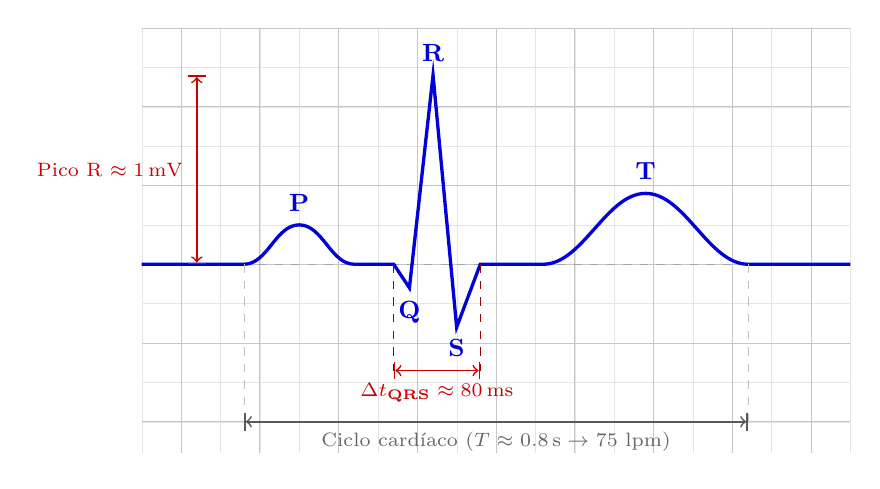
\begin{tikzpicture}[transform shape]
  % Cuadricula en tonos grises acorde a las graficas tecnicas del informe
  \draw[step=0.5, color=gray!20, line width=0.1pt] (-0.5, -2.4) grid (8.5, 3.0);
  \draw[step=1.0, color=gray!45, line width=0.25pt] (-0.5, -2.4) grid (8.5, 3.0);

  % Linea isoelectrica de referencia (0 V)
  \draw[dashed, color=gray!70, line width=0.5pt] (-0.5, 0) -- (8.5, 0);

  % Trazado de la senal de biopotencial ECG en azul (curva principal)
  \draw[color=blue!85!black, very thick, smooth] 
    (-0.5, 0) -- (0.8, 0) 
    .. controls (1.1, 0) and (1.2, 0.5) .. (1.5, 0.5)
    .. controls (1.8, 0.5) and (1.9, 0) .. (2.2, 0)
    -- (2.7, 0)
    -- (2.9, -0.3) % Q
    -- (3.2, 2.4)  % R
    -- (3.5, -0.8) % S
    -- (3.8, 0)    % Punto J
    -- (4.6, 0)
    .. controls (5.1, 0) and (5.4, 0.9) .. (5.9, 0.9)
    .. controls (6.4, 0.9) and (6.7, 0) .. (7.2, 0)
    -- (8.5, 0);

  % Identificacion clara de las ondas P, Q, R, S, T
  \node[above, font=\bfseries\small, color=blue!85!black] at (1.5, 0.55) {P};
  \node[below, font=\bfseries\small, color=blue!85!black] at (2.9, -0.35) {Q};
  \node[above, font=\bfseries\small, color=blue!85!black] at (3.2, 2.45) {R};
  \node[below=1pt, font=\bfseries\small, color=blue!85!black] at (3.5, -0.8) {S};
  \node[above, font=\bfseries\small, color=blue!85!black] at (5.9, 0.95) {T};

  % Cota vertical de amplitud de pico R (en rojo sutil)
  \draw[|<->|, semithick, color=red!80!black] (0.2, 0) -- (0.2, 2.4);
  \node[anchor=east, font=\scriptsize, color=red!80!black] at (0.15, 1.2) {Pico R $\approx \SI{1}{\milli\volt}$};

  % Cota de duracion temporal del complejo QRS (determina frecuencia de corte fH)
  \draw[dashed, color=red!60!black, line width=0.35pt] (2.7, 0) -- (2.7, -1.35);
  \draw[dashed, color=red!60!black, line width=0.35pt] (3.8, 0) -- (3.8, -1.35);
  \draw[|<->|, semithick, color=red!80!black] (2.7, -1.35) -- (3.8, -1.35);
  \node[below=1pt, font=\scriptsize\bfseries, color=red!80!black] at (3.25, -1.35) {$\Delta t_{\text{QRS}} \approx \SI{80}{\milli\second}$};

  % Cota del ciclo cardiaco completo (determina frecuencia fundamental f0)
  \draw[dashed, color=gray!50, line width=0.35pt] (0.8, 0) -- (0.8, -2.0);
  \draw[dashed, color=gray!50, line width=0.35pt] (7.2, 0) -- (7.2, -2.0);
  \draw[|<->|, semithick, color=gray!70!black] (0.8, -2.0) -- (7.2, -2.0)
    node[midway, below, font=\scriptsize, color=gray!80!black] {Ciclo cardíaco ($T \approx \SI{0.8}{\second} \rightarrow 75\ \text{lpm}$)};

\end{tikzpicture}
%
  \caption{Forma de onda un electrocardiograma (ondas P, QRS y T).}
  \label{fig:morfologia_ecg}
\end{figure}

El trazado característico de cada latido normal presenta tres componentes principales (Figura~\ref{fig:morfologia_ecg}):
\begin{itemize}
  \item \textbf{Onda P}: Pequeña deflexión inicial de baja frecuencia y amplitud reducida (típicamente entre $\SI{0.1}{\milli\volt}$ y $\SI{0.3}{\milli\volt}$).
  \item \textbf{Complejo QRS}: Señal de tipo pulsante rápida que concentra la mayor amplitud ($\sim \SI{1}{\milli\volt}$) y las componentes de mayor frecuencia del trazado, con una duración aproximada de $\SI{80}{\milli\second}$ a $\SI{120}{\milli\second}$.
  \item \textbf{Onda T}: Deflexión posterior más suave que marca el fin del ciclo de bombeo.
\end{itemize}

La tensión diferencial se obtiene conectando el electrodo del brazo izquierdo ($V_{\text{LA}}$) a la entrada no inversora y el electrodo del brazo derecho ($V_{\text{RA}}$) a la entrada inversora:
\begin{equation*}
  v_d = V_{\text{LA}} - V_{\text{RA}}
\end{equation*}

Se emplea además un electrodo de referencia conectado a la pierna derecha (RL), el cual se une a la masa analógica del instrumento para fijar el potencial del paciente respecto al circuito de medición.

\section{Desafíos Electrónicos en la Adquisición de la Señal}

El acondicionamiento analógico de biopotenciales presenta cuatro dificultades concretas que condicionan la arquitectura del circuito:
\begin{enumerate}
  \item \textbf{Muy baja amplitud útil}: La señal cardíaca diferencial sobre la piel tiene una amplitud de apenas $\SI{0.5}{\milli\volt\text{pp}}$ a $\SI{2}{\milli\volt\text{pp}}$. Por lo tanto, el circuito requiere una ganancia de tensión de al menos $1000\ \text{V/V}$ ($\SI{60}{\decibel}$) para entregar un nivel normalizado de $\SI{1}{\volt\text{pp}}$, apto para su visualización en osciloscopio o su digitalización mediante un conversor A/D.
  \item \textbf{Interferencia de red a $\SI{50}{\hertz}$}: El cuerpo humano actúa como una antena que capta campos electromagnéticos de la red eléctrica por acoplamiento capacitivo. Esta tensión de modo común puede superar los cientos de milivoltios (mucho mayor que la propia señal cardíaca), por lo que el amplificador debe ofrecer una Relación de Rechazo de Modo Común (RRMC) sumamente elevada ($\gg \SI{80}{\decibel}$) para cancelar dicha interferencia.
  \item \textbf{Tensión continua de contacto electrodo-piel}: El contacto entre el electrodo metálico y la piel con gel conductor genera una tensión galvánica continua de semicelda que puede alcanzar hasta $\pm \SI{300}{\milli\volt}$. Si esta continua se amplificara con la ganancia diferencial total, saturaría inmediatamente los amplificadores contra los rieles de alimentación. Por ello, el circuito debe poseer acoplamiento capacitivo o filtrado pasaaltos con corte en $f_L \approx \SI{0.05}{\hertz} - \SI{0.07}{\hertz}$ para bloquear la continua.
  \item \textbf{Alta impedancia de la piel}: La epidermis presenta una
      impedancia de contacto que suele ubicarse entre $\SI{5}{\kilo\ohm}$ y
        $\SI{100}{\kilo\ohm}$. Para evitar atenuación de la señal por efecto de
        carga resistiva, las entradas del amplificador deben presentar una
        impedancia de entrada muy alta ($Z_i \gg \SI{10}{\mega\ohm}$), lo que
        motiva el uso de amplificadores con transistores de efecto de campo
        (tecnología BiFET/JFET).
\end{enumerate}

\section{Selección del circuito a emplear}

Para dimensionar adecuadamente la solución circuital, conviene analizar por qué las topologías más simples resultan insuficientes para esta aplicación:

\begin{itemize}

  \item \textbf{Amplificador simple no inversor}: Como la interferencia de red a
      $\SI{50}{\hertz}$ captada por el cuerpo puede superar ampliamente la
        magnitud de la señal cardíaca, un amplificador simple referido a masa
        carece de capacidad de rechazo de modo común. Se requiere de forma obligatoria una topología
        diferencial.

  \item \textbf{Restador diferencial clásico de un solo operacional}: Un
      restador convencional presenta impedancias dispares ($R_1$ frente a $R_3 +
        R_4$) comparables a la impedancia piel-electrodo ($\SI{5}{\kilo\ohm}$ a
        $\SI{100}{\kilo\ohm}$). Esto genera atenuación por carga y provoca que
        cualquier desbalance entre electrodos
        rompa la simetría del puente, reduciendo el CMRR a valores inferiores a
        $\SI{40}{\decibel} - \SI{50}{\decibel}$.

  \item \textbf{Amplificador de Instrumentación}:

  \begin{enumerate}

      \item \textit{Impedancia de entrada muy alta en ambos terminales}: Las señales ingresan directamente a los
          terminales no inversores de los buffers $U_1$ y $U_2$.
    \item \textit{Amplificación diferencial selectiva }: La primera etapa entrega una ganancia diferencial elevada
          ($A_{vd1} = 1 + 2R_2/R_1$) mientras que atenúa el modo común.
    \item \textit{Ajuste de ganancia con un único resistor ($R_1$)}: Permite
        modificar o calibrar la amplificación global variando únicamente la
          resistencia central $R_1$, sin comprometer el balance del puente
          restador.
  \end{enumerate}
\end{itemize}

\section{Especificaciones de Diseño}

En función de los requerimientos analizados, el circuito a desarrollar debe cumplir con los parámetros fijados en el Cuadro~\ref{tab:especificaciones}.

\begin{table}[!ht]
  \centering
  \caption{Especificaciones impuestas para el diseño del amplificador de instrumentación.}
  \label{tab:especificaciones}
  \resizebox{\textwidth}{!}{%
  \begin{tabular}{|l|c|l|}
    \hline
    Parámetro & Valor de diseño & Justificación técnica \\ \hline
    Ganancia diferencial ($A_{md}$) & $\SI{60}{\decibel}$ ($1000\ \text{V/V}$) & Escala entrada de $\SI{1}{\milli\volt\text{pp}}$ a salida de $\SI{1}{\volt\text{pp}}$ \\ \hline
    Frecuencia de corte inferior ($f_L$) & $\SI{0.05}{\hertz}$ a $\SI{0.07}{\hertz}$ & Bloquea derivas de continua \\ \hline
    Frecuencia de corte superior ($f_H$) & $\SI{70}{\hertz}$ a $\SI{100}{\hertz}$ & Atenúa ruido muscular (EMG) e interferencias de alta frecuencia \\ \hline
    Rechazo de Modo Común (RRMC) & $\gg \SI{80}{\decibel}$ & Atenúa la interferencia de red de $\SI{50}{\hertz}$ \\ \hline
    Impedancia de entrada ($Z_i$) & $> \SI{5}{\mega\ohm}$ & Evita caída de tensión por impedancia de contacto del electrodo \\ \hline
    Acoplamiento interetapas & Corriente alterna (CA) & Bloquea corrimientos de offset y evita saturación \\ \hline
  \end{tabular}%
  }
\end{table}

\chapter{Desarrollo Teórico y Diseño del Circuito}
\label{sec:desarrollo_diseno}

\section{Amplificador de Instrumentación}

La arquitectura conceptual del amplificador de instrumentación de tres amplificadores operacionales (Figura~\ref{crkt:amp_inst_teorico}) se compone de dos etapas funcionales bien definidas: en primer lugar, una etapa de entrada diferencial con alta impedancia implementada mediante dos amplificadores operacionales ($U_1$ y $U_2$); en segundo lugar, una etapa restadora de precisión encargada de eliminar las señales de modo común, constituida por un tercer operacional ($U_3$).

\begin{figure}[!ht]
  \centering
    \begin{tikzpicture}[american, transform shape]

  % -------------------------------------------------------------
  % Entradas de señal (horizontales alineadas con los terminales +)
  % -------------------------------------------------------------
  % U1 con yscale=-1 tiene su terminal U1.+ en y = 2.99
  % U2 con yscale=1 tiene su terminal U2.+ en y = -2.99
  \node[ocirc] (in1) at (0.3, 2.99) {};
  \node[anchor=east] at (in1.west) {$e_1$};
  \node[ocirc] (in2) at (0.3, -2.99) {};
  \node[anchor=east] at (in2.west) {$e_2$};

  % -------------------------------------------------------------
  % Etapa 1: Buffers de entrada (U1 y U2)
  % -------------------------------------------------------------
  \node[op amp, yscale=-1] (U1) at (3.0, 2.5) {};
  \node at (2.8, 2.5) {$U_1$};
  \draw (in1) -- (U1.+);

  \node[op amp] (U2) at (3.0, -2.5) {};
  \node at (2.8, -2.5) {$U_2$};
  \draw (in2) -- (U2.+);

  % Nodos de terminales inversores
  \draw (U1.-) -- (1.8, 2.01);
  \draw (U2.-) -- (1.8, -2.01);

  % Impedancia Z1 entre terminales inversores
  \draw (1.8, 0.9) to[generic, l={$Z_1$}] (1.8, -0.9);
  \draw (1.8, 2.01) -- (1.8, 0.9);
  \draw (1.8, -2.01) -- (1.8, -0.9);

  % Impedancias de realimentacion Z2
  \draw (1.8, 1.3) node[circ]{} -- (2.3, 1.3)
        to[generic, l_={$Z_2$}] (3.7, 1.3)
        -- (4.2, 1.3) -- (4.2, 2.5) -- (U1.out);

  \draw (1.8, -1.3) node[circ]{} -- (2.3, -1.3)
        to[generic, l={$Z_2$}] (3.7, -1.3)
        -- (4.2, -1.3) -- (4.2, -2.5) -- (U2.out);

  % Tensiones intermedias eo1 y eo2
  \draw (U1.out) -- (4.8, 2.5) node[circ]{};
  \node[above] at (4.8, 2.5) {$e_{o1}$};
  \draw (U2.out) -- (4.8, -2.5) node[circ]{};
  \node[below] at (4.8, -2.5) {$e_{o2}$};

  % -------------------------------------------------------------
  % Etapa 2: Restador (U3)
  % -------------------------------------------------------------
  \node[op amp] (U3) at (9.0, 0.0) {};
  \node at (8.8, 0.0) {$U_3$};

  % Rama superior: eo1 -> Z3 -> entrada inversora U3.-
  \draw (4.8, 2.5) -- (5.0, 2.5)
        to[generic, l={$Z_3$}] (6.3, 2.5)
        -- (6.6, 2.5) |- (U3.-);

  % Rama inferior: eo2 -> Z3 -> entrada no inversora U3.+
  \draw (4.8, -2.5) -- (5.0, -2.5)
        to[generic, l_={$Z_3$}] (6.3, -2.5)
        -- (6.6, -2.5) |- (U3.+);

  % Realimentacion Z4 en lazo inversor (desde nodo antes de U3.- hacia U3.out)
  \draw (7.3, 0.49) node[circ]{} -- (7.3, 1.8)
        to[generic, l={$Z_4$}] (9.6, 1.8)
        -| (U3.out);
  \draw (9.6, 0.0) node[circ]{};

  % Impedancia Z4 a masa en lazo no inversor (desde nodo antes de U3.+ hacia masa)
  \draw (7.3, -0.49) node[circ]{}
        to[generic, l={$Z_4$}] (7.3, -1.9)
        node[ground]{};

  % Salida final eo
  \draw (U3.out) -- (10.6, 0.0);
  \node[ocirc] (eo) at (10.6, 0.0) {};
  \node[anchor=west] at (eo.east) {$e_o$};

\end{tikzpicture}
%
  \caption{Diagrama del circuito amplificador de instrumentación.}
  \label{crkt:amp_inst_teorico}
\end{figure}

El análisis del circuito se puede realizar a partir del estudio de cada etapa,
asumiendo amplificadores operacionales ideales en régimen lineal con
cortocircuito virtual ($v_- = v_+$) e impedancias de entrada infinitas.

En primer lugar, se analiza la segunda etapa correspondiente al restador diferencial de precisión ($U_3$) con sus impedancias balanceadas $Z_3$ y $Z_4$. Dado que la corriente de entrada al pin no inversor del operacional es nula, el potencial $v_{+3}$ queda determinado por el divisor de tensión pasivo conectado a la salida intermedia $e_{o2}$:
\begin{equation}
  v_{+3} = e_{o2} \cdot \frac{Z_4}{Z_3 + Z_4}
  \label{eq:paso1_vplus}
\end{equation}

Por otro lado, planteando la ley de corrientes de Kirchhoff en el nodo inversor $v_{-3}$ y considerando que tampoco entra corriente al pin inversor del amplificador:
\begin{equation*}
  \frac{e_{o1} - v_{-3}}{Z_3} + \frac{e_o - v_{-3}}{Z_4} = 0
\end{equation*}
Separando los términos para despejar la tensión de salida $e_o$:

\begin{equation*}
  \frac{e_o}{Z_4} = \frac{v_{-3}}{Z_4} + \frac{v_{-3}}{Z_3} - \frac{e_{o1}}{Z_3} = v_{-3} \left(\frac{1}{Z_4} + \frac{1}{Z_3}\right) - \frac{e_{o1}}{Z_3}
\end{equation*}
Multiplicando toda la igualdad por $Z_4$:
\begin{equation*}
  e_o = v_{-3} \left(1 + \frac{Z_4}{Z_3}\right) - e_{o1} \frac{Z_4}{Z_3}
\end{equation*}

\begin{equation*}
  e_o = v_{-3} \cdot \frac{Z_3 + Z_4}{Z_3} - e_{o1} \cdot \frac{Z_4}{Z_3}
\end{equation*}

Considerando la condición de cortocircuito virtual ($v_{-3} = v_{+3}$) y sustituyendo la tensión $v_{+3}$ obtenida previamente~\eqref{eq:paso1_vplus}:
\begin{equation*}
  e_o = \left(e_{o2} \cdot \frac{Z_4}{Z_3 + Z_4}\right) \cdot \left(\frac{Z_3 + Z_4}{Z_3}\right) - e_{o1} \cdot \frac{Z_4}{Z_3}
\end{equation*}
\begin{equation*}
  e_o = e_{o2} \cdot \frac{Z_4}{Z_3} - e_{o1} \cdot \frac{Z_4}{Z_3}
\end{equation*}
\begin{equation}
  e_o = (e_{o2} - e_{o1}) \cdot \frac{Z_4}{Z_3}
  \label{eq:eo_restador}
\end{equation}

Por su parte, en la primera etapa, las señales de entrada $e_1$ y $e_2$ ingresan
directamente a los terminales no inversores de los operacionales $U_1$ y $U_2$.
Por cortocircuito virtual ($v_{-1} = e_1$ y $v_{-2} = e_2$), sobre la impedancia
central $Z_1$ cae la diferencia $(e_1 - e_2)$, circulando una
corriente $i = (e_1 - e_2)/Z_1$ que fluye íntegramente a través de las ramas de
realimentación $Z_2$.

Para la componente diferencial, por simetría el punto medio de $Z_1$ se encuentra a potencial nulo (masa virtual de señal). Cada mitad del circuito queda así desacoplada con una impedancia equivalente $Z_1/2$ a masa, operando como una etapa no inversora con ganancia $1 + \frac{Z_2}{Z_1/2} = 1 + 2\frac{Z_2}{Z_1}$. Se obtienen así las expresiones desacopladas de las salidas intermedias:
\begin{equation*}
  e_{o2} = e_2 \cdot \left(1 + 2 \frac{Z_2}{Z_1}\right), \qquad e_{o1} = e_1 \cdot \left(1 + 2 \frac{Z_2}{Z_1}\right)
\end{equation*}
Restando miembro a miembro ambas salidas intermedias:
\begin{equation}
  e_{o2} - e_{o1} = (e_2 - e_1) \cdot \left(1 + 2 \frac{Z_2}{Z_1}\right)
  \label{eq:diff_salidas_etapa1}
\end{equation}

Luego, reemplazando la diferencia entre las salidas intermedias~\eqref{eq:diff_salidas_etapa1} en la ecuación del restador~\eqref{eq:eo_restador}, se obtiene la tensión de salida total del sistema:
\begin{equation*}
  e_o = (e_2 - e_1) \cdot \left(1 + 2 \frac{Z_2}{Z_1}\right) \cdot \frac{Z_4}{Z_3}
\end{equation*}
Dividiendo ambos miembros por la diferencia $(e_2 - e_1)$, se obtiene la ganancia diferencial de tensión del amplificador de instrumentación:
\begin{equation*}
  \frac{e_o}{e_2 - e_1} = \left(1 + 2 \frac{Z_2}{Z_1}\right) \cdot \frac{Z_4}{Z_3}
\end{equation*}

\section{Filtrado Pasabanda Activo}

El filtrado pasa banda suele implementarse como una etapa pasiva o activa independiente
a la salida del restador. No obstante, también se puede integrar la respuesta frecuencial
directamente en las redes de realimentación y entrada de la etapa restadora ($U_3$), según se ilustra en el circuito de
la Figura~\ref{crkt:sustitucion_z}.

\begin{figure}[!ht]
  \centering
  \resizebox{0.75\textwidth}{!}{%
    \begin{tikzpicture}[american, transform shape]

  % -------------------------------------------------------------
  % Entradas de señal (horizontales alineadas con los terminales +)
  % -------------------------------------------------------------
  % U1 con yscale=-1 tiene U1.+ en y = 3.29 (2.8 + 0.49)
  % U2 con yscale=1 tiene U2.+ en y = -3.29 (-2.8 - 0.49)
  \node[ocirc] (in1) at (0.5, 3.29) {};
  \node[anchor=east] at (in1.west) {$e_1$};
  \node[ocirc] (in2) at (0.5, -3.29) {};
  \node[anchor=east] at (in2.west) {$e_2$};

  % -------------------------------------------------------------
  % Etapa 1: Buffers con sustitucion Z1 -> R1, Z2 -> R2
  % -------------------------------------------------------------
  \node[op amp, yscale=-1] (U1) at (3.5, 2.8) {};
  \node at (3.3, 2.8) {$U_1$};
  \draw (in1) -- (U1.+);

  \node[op amp] (U2) at (3.5, -2.8) {};
  \node at (3.3, -2.8) {$U_2$};
  \draw (in2) -- (U2.+);

  % Terminales inversores
  \draw (U1.-) -- (2.3, 2.31);
  \draw (U2.-) -- (2.3, -2.31);

  % Sustitucion Z1 = R1
  \draw (2.3, 0.9) to[american resistor, l={$R_1$}] (2.3, -0.9);
  \draw (2.3, 2.31) -- (2.3, 0.9);
  \draw (2.3, -2.31) -- (2.3, -0.9);

  % Sustitucion Z2 = R2
  \draw (2.3, 1.5) node[circ]{} -- (2.8, 1.5)
        to[american resistor, l_={$R_2$}] (4.2, 1.5)
        -- (4.7, 1.5) -- (4.7, 2.8) -- (U1.out);

  \draw (2.3, -1.5) node[circ]{} -- (2.8, -1.5)
        to[american resistor, l={$R_2$}] (4.2, -1.5)
        -- (4.7, -1.5) -- (4.7, -2.8) -- (U2.out);

  % -------------------------------------------------------------
  % Etapa 2: Sustitucion Z3 -> C3 serie R3, Z4 -> R4 paralelo C4
  % -------------------------------------------------------------
  \node[op amp] (U3) at (11.0, 0.0) {};
  \node at (10.8, 0.0) {$U_3$};

  % Rama superior: Z3(s) = C3 serie R3 hacia entrada inversora U3.-
  \draw (U1.out) -- (5.2, 2.8) node[circ]{}
        to[C, l={$C_3$}] (6.6, 2.8)
        to[american resistor, l={$R_3$}] (8.3, 2.8)
        -- (8.8, 2.8) |- (U3.-);

  % Rama inferior: Z3(s) = C3 serie R3 hacia entrada no inversora U3.+
  \draw (U2.out) -- (5.2, -2.8) node[circ]{}
        to[C, l_={$C_3$}] (6.6, -2.8)
        to[american resistor, l_={$R_3$}] (8.3, -2.8)
        -- (8.8, -2.8) |- (U3.+);

  % Realimentacion Z4(s) = R4 paralelo C4 en lazo inversor
  \draw (9.5, 0.49) node[circ]{} -- (9.5, 2.3);
  \draw (9.5, 2.3) -- (9.8, 2.3) -- (9.8, 3.0)
        to[american resistor, l={$R_4$}] (11.8, 3.0)
        -- (11.8, 2.3);
  \draw (9.8, 2.3) -- (9.8, 1.6)
        to[C, l={$C_4$}] (11.8, 1.6)
        -- (11.8, 2.3);
  \draw (11.8, 2.3) -- (12.3, 2.3) -| (U3.out);
  \draw (12.3, 0.0) node[circ]{};

  % Red a masa no inversora Z4(s) = R4 paralelo C4
  \draw (9.5, -0.49) node[circ]{} -- (9.5, -1.3) -- (10.0, -1.3);
  \draw (10.0, -1.3) to[american resistor, l_={$R_4$}] (10.0, -2.6);
  \draw (10.0, -1.3) -- (11.4, -1.3)
        to[C, l={$C_4$}] (11.4, -2.6);
  \draw (10.0, -2.6) -- (11.4, -2.6);
  \draw (10.7, -2.6) node[circ]{} -- (10.7, -2.9) node[ground]{};

  % Salida filtrada e_o3
  \draw (U3.out) -- (13.0, 0.0);
  \node[ocirc] (eo3) at (13.0, 0.0) {};
  \node[anchor=west] at (eo3.east) {$e_{o3}$};

\end{tikzpicture}
%
    }
  \caption{Topología del amplificador de instrumentación con las impedancias actualizadas para filtrado pasabanda activo.}
  \label{crkt:sustitucion_z}
\end{figure}

Para ello se efectúan las siguientes sustituciones de componentes en el dominio de Laplace:
\begin{itemize}
  \item $Z_1 = R_1$: Resistencia que calibra la ganancia diferencial de entrada.
  \item $Z_2 = R_2$: Resistencias de simetría en los lazos de realimentación de $U_1$ y $U_2$.
  \item $Z_3(s)$: Rama de entrada al restador, compuesta por la conexión serie de un capacitor $C_3$ y un resistor $R_3$:
  \begin{equation}
    Z_3(s) = R_3 + \frac{1}{s C_3} = \frac{s R_3 C_3 + 1}{s C_3}
    \label{eq:z3_s}
  \end{equation}
  \item $Z_4(s)$: Rama de realimentación e impedancia a masa, formada por la conexión en paralelo de un resistor $R_4$ y
  un capacitor $C_4$:
  \begin{equation}
    Z_4(s) = R_4 \parallel \frac{1}{s C_4} = \frac{R_4}{s R_4 C_4 + 1}
    \label{eq:z4_s}
  \end{equation}
\end{itemize}

Para preservar el balance del restador y garantizar la máxima atenuación de modo común, las dos ramas de entrada al
operacional $U_3$ deben ser rigurosamente idénticas ($Z_3 = Z'_3$ y $Z_4 = Z'_4$). Bajo esta condición de puente balanceado
y aplicando en el dominio transformado de Laplace la relación del restador deducida en~\eqref{eq:eo_restador}, la salida de
la etapa $U_3$ viene dada por:
\begin{equation}
  e_{o3}(s) = (e_{o2}(s) - e_{o1}(s)) \frac{Z_4(s)}{Z_3(s)}
  \label{eq:salida_u3}
\end{equation}

Dividiendo las ecuaciones de impedancia~\eqref{eq:z4_s} y~\eqref{eq:z3_s}:
\begin{equation*}
  \frac{Z_4(s)}{Z_3(s)} = \frac{\dfrac{R_4}{s R_4 C_4 + 1}}{\dfrac{s R_3 C_3 + 1}{s C_3}} = \frac{s R_4 C_3}{(s R_3 C_3 + 1)(s R_4 C_4 + 1)}
\end{equation*}

Sustituyendo la diferencia de la primera etapa~\eqref{eq:diff_salidas_etapa1} en~\eqref{eq:salida_u3}, se arriba a la
función de transferencia analítica completa de las etapas 1 y 2:
\begin{equation}
  F(s) = \frac{e_{o3}(s)}{e_2(s) - e_1(s)} = \left(1 + 2 \frac{R_2}{R_1}\right) \frac{s R_4 C_3}{(s R_3 C_3 + 1)(s R_4 C_4 + 1)}
  \label{eq:ft_completa}
\end{equation}

\section{Análisis en Frecuencia y Diagrama de Bode}

La función de transferencia $F(s)$ formulada en la ecuación~\eqref{eq:ft_completa} revela de forma directa las singularidades
que moldean la respuesta en frecuencia:
\begin{enumerate}
  \item Cero en el origen ($s = 0$): Proporcionado por el término $s R_4 C_3$ en el numerador, introduce una asíntota de
  crecimiento de $+20\ \text{dB/década}$ desde frecuencias nulas. Esto asegura que la ganancia a corriente continua sea
  nula ($F(0) = 0$), eliminando por completo cualquier tensión de offset de entrada o potencial de contacto electrodo-piel.
  \item Polo inferior ($p_3$): Determinado por la constante de tiempo de la red serie de entrada:
  \begin{equation*}
    p_3 = \frac{1}{R_3 C_3} \implies f_L \approx \frac{p_3}{2 \pi} = \frac{1}{2 \pi R_3 C_3}
  \end{equation*}
  A partir de $f_L$, la respuesta cambia de $+20\ \text{dB/década}$ a pendiente horizontal ($0\ \text{dB/década}$),
  dando inicio a la banda pasante.
  \item Polo superior ($p_4$): Establecido por la constante de tiempo de la red en paralelo de realimentación:
  \begin{equation*}
    p_4 = \frac{1}{R_4 C_4} \implies f_H \approx \frac{p_4}{2 \pi} = \frac{1}{2 \pi R_4 C_4}
  \end{equation*}
  A partir de $f_H$, la respuesta cae con una pendiente asintótica de $-20\ \text{dB/década}$, atenuando interferencias de
  alta frecuencia.
\end{enumerate}

En la Figura~\ref{plot:bode_teorico} se ilustra el comportamiento frecuencial resultante, integrando el trazado asintótico ideal con la curva de respuesta real suavizada para la banda de paso delimitada entre $f_L$ y $f_H$.

\begin{figure}[!ht]
  \centering
  \resizebox{0.82\textwidth}{!}{%
    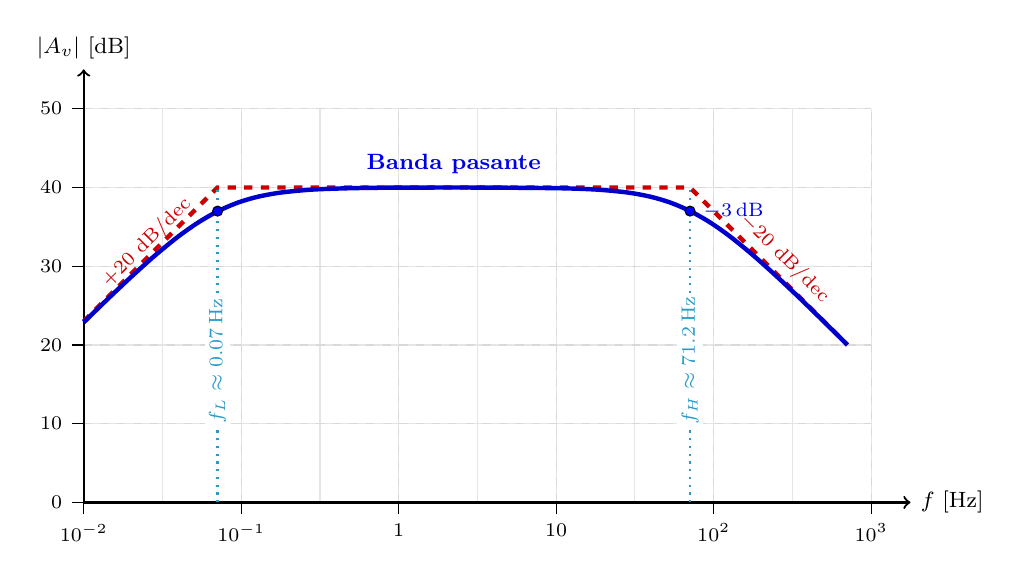
\begin{tikzpicture}[scale=1.0, transform shape]

  % Grid semilogaritmico tenue
  \draw[step=1.0, color=gray!20, thin] (0, 0) grid (10, 5);

  % Lineas de la grilla (SOLO para y > 0 y x > 0 para no superponer lineas punteadas sobre los ejes)
  \foreach \y in {1, 2, 3, 4, 5} {
    \draw[dashed, color=gray!30] (0, \y) -- (10, \y);
  }
  \foreach \x in {2, 4, 6, 8, 10} {
    \draw[dashed, color=gray!30] (\x, 0) -- (\x, 5);
  }

  % Marcas eje Y (Ganancia en dB)
  \foreach \y/\val in {0/0, 1/10, 2/20, 3/30, 4/40, 5/50} {
    \draw (0, \y) -- (-0.15, \y) node[left, font=\scriptsize] {$\val$};
  }

  % Marcas eje X (Decadas logaritmicas)
  \foreach \x/\label in {0/{$10^{-2}$}, 2/{$10^{-1}$}, 4/{$1$}, 6/{$10$}, 8/{$10^2$}, 10/{$10^3$}} {
    \draw (\x, 0) -- (\x, -0.15) node[below, font=\scriptsize] {\label};
  }

  % Ejes coordenados (dibujados solidos por encima de la grilla)
  \draw[->, thick] (0, 0) -- (10.5, 0) node[right, font=\footnotesize] {$f\ [\unit{\hertz}]$};
  \draw[->, thick] (0, 0) -- (0, 5.5) node[above, font=\footnotesize] {$|A_v|\ [\unit{\decibel}]$};

  % Curva Asintotica (linea discontinua roja)
  % fL = 0.071 Hz -> x_L = 2*(log10(0.071) + 2) = 1.70
  % fH = 71.18 Hz -> x_H = 2*(log10(71.18) + 2) = 7.70
  % Pendiente +20 dB/dec -> +1 por cada unidad de x
  \draw[dashed, ultra thick, red!80!black] 
    (0, 2.3) -- (1.70, 4.0) -- (7.70, 4.0) -- (9.70, 2.0);

  % Curva Real Suavizada (linea solida azul calculada analiticamente)
  \draw[ultra thick, blue!80!black] plot[smooth] coordinates {
    (0.00, 2.287) (0.30, 2.579) (0.60, 2.862) (0.90, 3.132) (1.20, 3.377) 
    (1.45, 3.553) (1.70, 3.697) (1.95, 3.805) (2.20, 3.880) (2.50, 3.935) 
    (2.90, 3.973) (3.40, 3.991) (4.00, 3.998) (5.00, 3.999) (6.00, 3.991) 
    (6.50, 3.974) (6.90, 3.937) (7.20, 3.882) (7.45, 3.808) (7.70, 3.701) 
    (7.95, 3.559) (8.20, 3.384) (8.50, 3.140) (8.80, 2.871) (9.10, 2.588) 
    (9.40, 2.296) (9.70, 2.000)
  };

  % Lineas de corte y singularidades con etiquetas verticales sobre las lineas
  \draw[dotted, thick, color=cyan!80!black] (1.70, 0) -- (1.70, 4.0);
  \node[fill=white, inner sep=1.5pt, font=\scriptsize, text=cyan!80!black, rotate=90] at (1.70, 1.8) {$f_L \approx \SI{0.07}{\hertz}$};

  \draw[dotted, thick, color=cyan!80!black] (7.70, 0) -- (7.70, 4.0);
  \node[fill=white, inner sep=1.5pt, font=\scriptsize, text=cyan!80!black, rotate=90] at (7.70, 1.8) {$f_H \approx \SI{71.2}{\hertz}$};

  % Anotaciones de pendientes y ganancias
  \node[above, font=\footnotesize\bfseries, color=blue!90!black] at (4.7, 4.05)
    {Banda pasante};
  \node[font=\scriptsize, color=red!80!black, rotate=45] at (0.8, 3.3) {$+20\ \text{dB/dec}$};
  \node[font=\scriptsize, color=red!80!black, rotate=-45] at (8.9, 3.1) {$-20\ \text{dB/dec}$};

  % Punto de -3dB
  \draw[fill=blue] (1.70, 3.7) circle (1.8pt);
  \draw[fill=blue] (7.70, 3.7) circle (1.8pt);
  \node[right, font=\scriptsize, color=blue!90!black] at (7.75, 3.7) {$-\SI{3}{\decibel}$};

\end{tikzpicture}
%
  }
  \caption{Respuesta en frecuencia del circuito pasabanda.}
  \label{plot:bode_teorico}
\end{figure}

La función de transferencia~\eqref{eq:ft_completa} se puede reescribir en su forma canónica de Bode agrupando los factores del numerador:
\begin{equation*}
  F(s) = \frac{K \cdot s}{\left(1 + \dfrac{s}{p_3}\right)\left(1 + \dfrac{s}{p_4}\right)}
\end{equation*}
donde los polos están dados por $p_3 = \dfrac{1}{R_3 C_3}$ y $p_4 = \dfrac{1}{R_4 C_4}$, y la constante de escala del numerador $K$ se define analíticamente como:
\begin{equation}
    K = \left(1 + 2 \frac{R_2}{R_1}\right) (R_3 C_3) \quad \mbox{(considerando $R_4 = R_3$)}
    \label{eq:definicion_k}
\end{equation}


Para analizar el efecto de esta constante K, se evalúa la función de
transferencia en el rango de frecuencias intermedias que delimitan la
banda de paso ($p_3 \ll \omega \ll p_4$):

\begin{itemize}
  \item En el polo inferior, dado que $\omega \gg p_3$, se cumple: $1 + \dfrac{s}{p_3} \approx \dfrac{s}{p_3}$.
  \item En el polo superior, dado que $\omega \ll p_4$, se cumple: $1 + \dfrac{s}{p_4} \approx 1$.
\end{itemize}
Sustituyendo ambas aproximaciones en la expresión canónica de $F(s)$:
\begin{equation*}
  F(s) \approx \frac{K \cdot s}{\left(\dfrac{s}{p_3}\right) \cdot 1} = K \cdot p_3
\end{equation*}
finalmente,
\begin{equation*}
  K \cdot p_3 = \left(1 + 2 \frac{R_2}{R_1}\right) R_3 C_3 \cdot \frac{1}{R_3
    C_3} =
\end{equation*}
\begin{equation}
    = 1 + 2 \frac{R_2}{R_1} = K_{1-2}
    \label{eq:k_final}
\end{equation}

Por lo tanto, se puede observar que la amplificación intermedia depende de las resistencias de
la etapa diferencial.

\section{Determinación de componentes}

La selección de capacitores comerciales es más restringida que la de resistores. Por
este motivo, se comienza fijando en primer lugar los valores comerciales de los
capacitores y, en base a ellos y a las frecuencias de corte, se determinan los
valores resistivos del circuito:

\begin{enumerate}
  \item Frecuencias de corte de proyecto:

    A partir de las exigencias de diseño para eliminar derivas de baja frecuencia
    y ruidos electromagnéticos de alta frecuencia, se establecen las
    frecuencias de corte objetivo:
  \begin{align*}
    f_L &\approx \SI{0.07}{\hertz} \implies p_3 = 2\pi f_L \approx \SI{0.4545}{\radian/\second} \\
    f_H &\approx \SI{72}{\hertz} \implies p_4 = 2\pi f_H \approx \SI{454.55}{\radian/\second}
  \end{align*}

  \item Selección inicial de capacitores comerciales ($C_4$ y $C_3$):
  \begin{itemize}
    \item Para la fijación del polo superior ($p_4$), se selecciona un capacitor comercial de poliéster de:
    \begin{equation*}
      C_4 = \SI{2.2}{\nano\farad}
    \end{equation*}
    \item Para la fijación del polo inferior ($p_3$):
    \begin{equation*}
      C_3 = \SI{2.2}{\micro\farad}
    \end{equation*}
  \end{itemize}

  \item Determinación de las resistencias del restador y filtrado ($R_4$ y $R_3$):
  Con los valores de capacidad ya adoptados, se despejan analíticamente las resistencias requeridas:
  \begin{itemize}
    \item A partir de la constante de tiempo del polo superior $p_4 = 1 / (R_4 C_4)$, se calcula $R_4$:
    \begin{equation*}
      R_4 = \frac{1}{p_4 C_4} = \frac{1}{454.55 \times 2.2 \times 10^{-9}} \approx \SI{1.000}{\mega\ohm}
    \end{equation*}
    Se adopta el valor comercial normalizado de  $\SI{1}{\mega\ohm}$ al $1\%$.
    \item Para garantizar la simetría y el balance óptimo del puente restador de $U_3$ (requisito esencial para maximizar el RRMC de la segunda etapa), se impone por diseño la igualdad de resistencias $R_3 = R_4$:
    \begin{equation*}
      R_3 = \SI{1}{\mega\ohm}\ (1\%)
    \end{equation*}
    Verificando con el capacitor $C_3 = \SI{2.2}{\micro\farad}$ previamente seleccionado, la frecuencia de corte inferior resultante es:
    \begin{equation*}
      f_L = \frac{1}{2\pi R_3 C_3} = \frac{1}{2\pi \times 10^6 \times 2.2 \times 10^{-6}} \approx \SI{0.0723}{\hertz}
    \end{equation*}
    la cual satisface el requerimiento de $\SI{0.07}{\hertz}$.
  \end{itemize}

  \item Ganancia diferencial de primera etapa ($R_1$ y $R_2$): Fijando los resistores de realimentación de los buffers de entrada en un valor
        de $R_2 = \SI{100}{\kilo\ohm}$ al $1\%$ y con la constante de tiempo del
        polo inferior fijada por $R_3 = \SI{1}{\mega\ohm}$ y $C_3 =
        \SI{2.2}{\micro\farad}$ ($p_3 \approx \SI{0.4545}{\radian/\second}$), se
        utiliza la expresión deducida en~\eqref{eq:k_final} para obtener la
        ganancia provista por la etapa de entrada
        ($K_{1-2} = 1 + 2 R_2/R_1$).

  Adoptando para la resistencia de ganancia el valor comercial normalizado de $R_1 = \SI{4.7}{\kilo\ohm}$
  \begin{equation*}
    K_{1-2} = 1 + 2 \frac{R_2}{R_1} = 1 + 2 \frac{\SI{100}{\kilo\ohm}}{\SI{4.7}{\kilo\ohm}} \approx 43.55\ \text{V/V} \equiv \SI{32.78}{\decibel}
  \end{equation*}
\end{enumerate}

\section{Etapa de Salida y Ajuste de Ganancia Global}

La especificación de diseño exige una ganancia diferencial global mínima de
$A_{\text{total}} \ge \SI{60}{\decibel}$ ($1000\ \text{V/V}$). Por lo tanto, se
requiere una etapa final para obtener esta amplificación que falta. Para ello,
se emplea un amplificador en configuración no inversor, cuya ganancia está dada
por:
\begin{equation*}
  A_{v4} = 1 + \frac{R_8}{R_9}
\end{equation*}

Conociendo que las etapas de entrada y filtrado aportan una ganancia intermedia
de $K_{1-2} \approx 43.55\ \text{V/V}$ ($\SI{32.78}{\decibel}$), la ganancia
mínima que debe proporcionar la etapa final de amplificación adicional es:

\begin{equation*}
  A_{v4,\text{mín}} = \frac{A_{\text{total}}}{K_{1-2}} \ge \frac{1000\ \text{V/V}}{43.55\ \text{V/V}} \approx 22.96\ \text{V/V} \equiv \SI{27.22}{\decibel}
\end{equation*}

Se seleccionan $R_8 = \SI{220}{\kilo\ohm}$ y $R_9 = \SI{7}{\kilo\ohm}$:

\begin{equation*}
  A_{v4} = 1 + \frac{\SI{220}{\kilo\ohm}}{\SI{7}{\kilo\ohm}} = 1 + 31.43 = 32.43\ \text{V/V} \equiv \SI{30.22}{\decibel}
\end{equation*}

Así, la ganancia global nominal del circuito en la banda de paso intermedia resulta:
\begin{equation*}
  A_{\text{total}} = K_{1-2} \cdot A_{v4} = 43.55 \times 32.43 \approx 1412.3\ \text{V/V} \equiv \SI{63.0}{\decibel}
\end{equation*}

De este modo, una señal cardíaca de entrada superficial de $\SI{1}{\milli\volt\text{pp}}$ se amplifica hasta alcanzar más de $\SI{1}{\volt\text{pp}}$ en el terminal $V_o$, nivel ideal para su adquisición directa y procesamiento digital.

\section{Esquema Eléctrico Completo del Amplificador}

En la Figura~\ref{crkt:amplificador_completo} se presenta el esquema eléctrico completo del amplificador de
instrumentación con filtrado pasabanda y etapa de ajuste de ganancia.
\begin{figure}[!ht]
  \centering
  \resizebox{0.98\textwidth}{!}{%
    \begin{tikzpicture}[american, scale=0.76, transform shape]

  % =============================================================
  % 1. ENTRADAS DE SENAL DIRECTAS (HORIZONTALES)
  % =============================================================
  % U1 con yscale=-1 tiene U1.+ en y = 2.99
  % U2 con yscale=1 tiene U2.+ en y = -2.99
  \node[ocirc] (in1) at (-0.5, 2.99) {};
  \node[anchor=east] at (in1.west) {$e_1\text{ (LA)}$};
  \node[ocirc] (in2) at (-0.5, -2.99) {};
  \node[anchor=east] at (in2.west) {$e_2\text{ (RA)}$};

  % =============================================================
  % 2. ETAPA 1: BUFFER DIFERENCIAL (U1 y U2)
  % =============================================================
  % U1 (superior, yscale=-1)
  \node[op amp, yscale=-1] (U1) at (2.2, 2.5) {};
  \node at (2.0, 2.5) {$U_1$};
  \draw (in1) -- (U1.+);

  % U2 (inferior)
  \node[op amp] (U2) at (2.2, -2.5) {};
  \node at (2.0, -2.5) {$U_2$};
  \draw (in2) -- (U2.+);

  % Entradas inversoras hacia barra central
  \draw (U1.-) -- (1.0, 2.01);
  \draw (U2.-) -- (1.0, -2.01);

  % Resistencia de ganancia R1
  \draw (1.0, 2.01) -- (1.0, 0.9)
        to[american resistor, l={$R_1$}] (1.0, -0.9)
        -- (1.0, -2.01);

  % Realimentacion R2 de U1
  \draw (1.0, 1.4) node[circ]{} -- (1.5, 1.4)
        to[american resistor, l_={$R_2$}] (2.9, 1.4)
        -- (3.4, 1.4) -- (3.4, 2.5) -- (U1.out);

  % Realimentacion R2 de U2
  \draw (1.0, -1.4) node[circ]{} -- (1.5, -1.4)
        to[american resistor, l={$R_2$}] (2.9, -1.4)
        -- (3.4, -1.4) -- (3.4, -2.5) -- (U2.out);

  % =============================================================
  % 3. ETAPA 2: RESTADOR Y FILTRO PASABANDA ACTIVO (U3)
  % =============================================================
  \node[op amp] (U3) at (12.6, 0.0) {};
  \node at (12.4, 0.0) {$U_3$};

  % Rama superior: U1.out -> C3 serie R3 -> U3.-
  \draw (U1.out) -- (4.0, 2.5) node[circ]{}
        to[C, l={$C_3$}] (5.8, 2.5)
        -- (6.9, 2.5)
        to[american resistor, l={$R_3$}] (9.1, 2.5)
        -- (10.0, 2.5) |- (U3.-);

  % Rama inferior: U2.out -> C3 serie R3 -> U3.+
  \draw (U2.out) -- (4.0, -2.5) node[circ]{}
        to[C, l_={$C_3$}] (5.8, -2.5)
        -- (6.9, -2.5)
        to[american resistor, l_={$R_3$}] (9.1, -2.5)
        -- (10.0, -2.5) |- (U3.+);

  % Realimentacion en lazo inversor: R4 || C4
  % U3.- esta en (11.4, 0.49). Derivamos el lazo en x = 10.7
  \draw (10.7, 0.49) node[circ]{} -- (10.7, 2.4) -- (11.2, 2.4);
  % Rama R4 (superior)
  \draw (11.2, 2.4) -- (11.2, 3.2)
        to[american resistor, l={$R_4$}] (13.6, 3.2)
        -- (13.6, 2.4);
  % Rama C4 (inferior)
  \draw (11.2, 2.4) -- (11.2, 1.6)
        to[C, l={$C_4$}] (13.6, 1.6)
        -- (13.6, 2.4);
  % Cierre vertical limpio hacia la salida de U3
  \draw (13.6, 2.4) -- (14.4, 2.4) -- (14.4, 0.0);

  % Red no inversora a masa: R4 || C4
  % U3.+ esta en (11.4, -0.49). Derivamos en x = 10.7 hacia abajo
  \draw (10.7, -0.49) node[circ]{} -- (10.7, -1.3) -- (11.6, -1.3);
  % Rama R4 (vertical)
  \draw (11.6, -1.3) to[american resistor, l_={$R_4$}] (11.6, -2.8);
  % Rama C4 (vertical paralela)
  \draw (11.6, -1.3) -- (13.3, -1.3)
        to[C, l={$C_4$}] (13.3, -2.8);
  \draw (11.6, -2.8) -- (13.3, -2.8);
  \draw (12.45, -2.8) node[circ]{} -- (12.45, -3.2) node[ground]{};

  % =============================================================
  % 4. ETAPA 3: AMPLIFICADOR NO INVERSOR DE SALIDA (U4)
  % =============================================================
  \node[op amp] (U4) at (17.8, 0.0) {};
  \node at (17.6, 0.0) {$U_4$};

  % Salida de U3 hacia entrada no inversora de U4 con conexion limpia en x = 14.4
  \draw (U3.out) -- (14.4, 0.0) node[circ]{} -- (15.4, 0.0) |- (U4.+);

  % Realimentacion R8 para U4
  \draw (U4.out) -- (19.8, 0.0) node[circ]{} -- (19.8, 1.8)
        to[american resistor, l_={$R_8$}] (17.0, 1.8)
        -| (U4.-);
  \draw (17.0, 0.49) node[circ]{};

  % Red de ganancia a tierra: R9
  \draw (17.0, 1.8) -- (17.0, 2.4)
        to[american resistor, l_={$R_9$}] (17.0, 3.8)
        node[ground, yscale=-1]{};

  % Resistor de carga de salida a tierra: RL
  \draw (19.8, 0.0) -- (20.7, 0.0) node[circ]{};
  \draw (20.7, 0.0) to[american resistor, l={$R_L$}] (20.7, -1.6) node[ground]{};

  % Terminal de salida final
  \draw (20.7, 0.0) -- (21.8, 0.0);
  \node[ocirc] (vout) at (21.8, 0.0) {};
  \node[anchor=west] at (vout.east) {$V_o$};

\end{tikzpicture}
%
  }
  \caption{Esquema eléctrico completo del amplificador de instrumentación.}
  \label{crkt:amplificador_completo}
\end{figure}

En la Tabla~\ref{tab:componentes_finales} se listan todos los componentes del diseño con sus respectivas tolerancias y
funciones dentro del sistema.

\begin{table}[!ht]
  \centering
  \caption{Listado y especificación de componentes del circuito amplificador de instrumentación.}
  \label{tab:componentes_finales}
  \resizebox{\textwidth}{!}{%
  \begin{tabular}{|l|c|l|}
    \hline
    Componente & Valor nominal & Función en el circuito \\ \hline
    $R_1$ & $\SI{4.7}{\kilo\ohm}$ & Fijación de la ganancia diferencial de la etapa 1 \\ \hline
    $R_2$ ($\times 2$) & $\SI{100}{\kilo\ohm}$ & Simetría y ganancia del lazo de entrada \\ \hline
    $R_3$ ($\times 2$) & $\SI{1}{\mega\ohm}$ & Determinación del polo inferior y entrada al restador \\ \hline
    $R_4$ ($\times 2$) & $\SI{1}{\mega\ohm}$ & Determinación del polo superior y balance del restador \\ \hline
    $R_8$ & $\SI{220}{\kilo\ohm}$ & Realimentación de la etapa no inversora de salida \\ \hline
    $R_9$ & $\SI{7}{\kilo\ohm}$ & Resistor de fijación y ajuste de ganancia en $U_4$ \\ \hline
    $R_{10}$ ($R_L$) & $\SI{10}{\kilo\ohm}$ & Resistencia de carga nominal a tierra \\ \hline
    $C_3$ ($\times 2$) & $\SI{2.2}{\micro\farad}$ & Bloqueo galvánico de CC y fijación de $f_L$ \\ \hline
    $C_4$ ($\times 2$) & $\SI{2.2}{\nano\farad}$ & Filtro antialiasing activo y fijación de $f_H$ \\ \hline
    $U_1 - U_4$ & TL084 & Dispositivos activos de procesamiento analógico \\ \hline
  \end{tabular}%
  }
\end{table}

La realización física del circuito sobre placa de circuito impreso (PCB) para su ensayo en banco de trabajo se exhibe en el Capítulo~\ref{sec:simulacion_mediciones} (Figura~\ref{fig:crkt_implementado}), donde se analizan en detalle las mediciones experimentales y su contraste con los valores calculados y simulados.

\chapter{Simulación Circuital y Ensayos Experimentales}
\label{sec:simulacion_mediciones}

El presente capítulo aborda la validación del amplificador de instrumentación
diseñado a través de dos etapas complementarias: en primer lugar, la simulación
circuital para corroborar el modelo analítico en condiciones nominales; en
segundo lugar, el ensayo en laboratorio sobre la placa física implementada, a
fin de contrastar y comprobar los resultados esperados
frente al comportamiento real.

% =========================================================================
% PARTE 1: SIMULACIÓN CIRCUITAL
% =========================================================================
\section{Simulación Circuital}
\label{subsec:simulacion_ltspice}

Para evaluar el diseño analítico se implementó el circuito
completo en el software de simulación LTspice, empleando los modelos
provistos por Texas Instruments para la familia TL081/TL084
(\texttt{TL081.301}).

\subsection{Respuesta Temporal en Modo Diferencial}
A fin de evaluar la ganancia diferencial en la zona central plana de la banda pasante, se inyecta entre los terminales $e_1$ y $e_2$ una señal senoidal pura de amplitud $v_d = \SI{10}{\milli\volt}$ ($v_{d,\text{pp}} = \SI{20}{\milli\volt\text{pp}}$) a una frecuencia de $\SI{25}{\hertz}$. 

En la Figura~\ref{fig:sim_modo_dif} se presentan el circuito esquemático configurado en LTspice y la respuesta temporal en régimen permanente obtenida en el nodo de salida $V_o$.

\begin{figure}[!ht]
  \centering
  \begin{subfigure}[b]{0.88\textwidth}
    \centering
    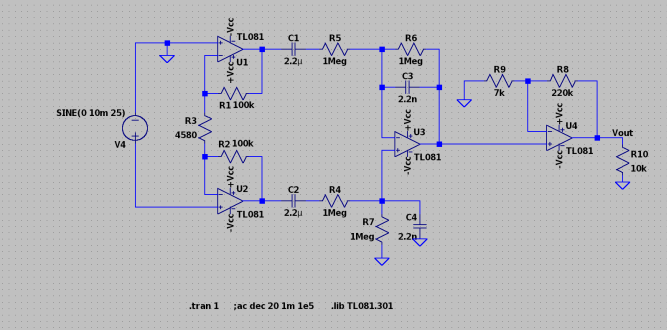
\includegraphics[width=\textwidth]{images/sim_crkt-modo_dif.png}
    \caption{Esquemático del circuito configurado en LTspice para excitación senoidal diferencial ($v_d = \SI{10}{\milli\volt}$, $f = \SI{25}{\hertz}$).}
    \label{subfig:sim_crkt_modo_dif}
  \end{subfigure}
  \vspace{0.4cm}
  \begin{subfigure}[b]{0.88\textwidth}
    \centering
    \resizebox{\linewidth}{!}{%
      \begin{tikzpicture}
  \pgfplotsset{
    scale only axis,
    xmin=0, xmax=120,
    xtick={0, 20, 40, 60, 80, 100, 120},
  }
  \begin{axis}[
    width=0.80\textwidth,
    height=5.2cm,
    grid=both,
    grid style={line width=.1pt, draw=gray!25},
    major grid style={line width=.2pt, draw=gray!45},
    xlabel={Tiempo [\unit{\milli\second}]},
    ylabel={Tensión diferencial de entrada $v_d$ [\unit{\milli\volt}]},
    ylabel style={color=red!80!black},
    yticklabel style={color=red!80!black},
    ymin=-30, ymax=40,
    ytick={-30, -20, -10, 0, 10, 20, 30, 40},
    axis y line*=left,
  ]
    \addplot[thick, dashed, color=red!80!black] table [x expr=\thisrow{time}*1000, y expr=\thisrow{vin}*1000] {sources/sim/sim_plot-ganancia_modo_dif.txt};
  \end{axis}
  \begin{axis}[
    width=0.80\textwidth,
    height=5.2cm,
    ylabel={Tensión de salida $V_o$ [\unit{\volt}]},
    ylabel style={color=blue!80!black},
    yticklabel style={color=blue!80!black},
    ymin=-18, ymax=24,
    ytick={-18, -12, -6, 0, 6, 12, 18, 24},
    axis y line*=right,
    axis x line=none,
    legend style={at={(0.98,0.95)}, anchor=north east, font=\footnotesize}
  ]
    \addlegendimage{thick, dashed, color=red!80!black}
    \addlegendentry{Entrada $v_d$ [\unit{\milli\volt}]}
    \addplot[thick, color=blue!85!black] table [x expr=\thisrow{time}*1000, y=vout] {sources/sim/sim_plot-ganancia_modo_dif.txt};
    \addlegendentry{Salida $V_o$ [\unit{\volt}]}
  \end{axis}
\end{tikzpicture}
%
    }
    \caption{Respuesta temporal en régimen permanente a $\SI{25}{\hertz}$.}
    \label{subfig:plot_sim_modo_dif}
  \end{subfigure}
  \caption{Simulación circuital y formas de onda del ensayo en modo diferencial a $\SI{25}{\hertz}$.}
  \label{fig:sim_modo_dif}
\end{figure}

Para la entrada diferencial aplicada de $\SI{10}{\milli\volt}$, la salida entrega una onda senoidal pura sin distorsión armónica con una amplitud de $v_{od} = \SI{13.36}{\volt}$ ($v_{od,\text{pp}} = \SI{26.73}{\volt\text{pp}}$), lo que determina una ganancia diferencial de:
\begin{equation*}
  A_{md,\text{sim}} = \frac{v_{od}}{v_d} = \frac{\SI{13.36}{\volt}}{\SI{10}{\milli\volt}} \approx 1336.3\ \text{V/V} \equiv \SI{62.52}{\decibel}
\end{equation*}

\subsection{Respuesta en Modo Común y Rechazo de Modo Común (RRMC)}
Para caracterizar la respuesta frente a interferencias de modo común (tales como la inducción capacitiva de la red de $\SI{50}{\hertz}$), se unen ambas entradas ($e_1 = e_2 = v_c$) y se aplica una señal senoidal de amplitud $v_c = \SI{1}{\volt}$ ($v_{c,\text{pp}} = \SI{2}{\volt\text{pp}}$) a $\SI{25}{\hertz}$.

En la Figura~\ref{fig:sim_modo_comun} se exhiben el esquemático de simulación correspondiente y la traza de tensión obtenida en la salida.

\begin{figure}[!ht]
  \centering
  \begin{subfigure}[b]{0.88\textwidth}
    \centering
    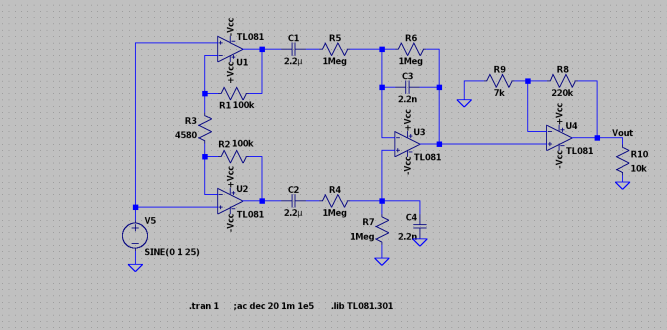
\includegraphics[width=\textwidth]{images/sim_crkt-modo_comun.png}
    \caption{Esquemático en LTspice configurado para modo común con entradas cortocircuitadas ($v_c = \SI{1}{\volt}$, $f = \SI{25}{\hertz}$).}
    \label{subfig:sim_crkt_modo_comun}
  \end{subfigure}
  \vspace{0.4cm}
  \begin{subfigure}[b]{0.88\textwidth}
    \centering
    \resizebox{\linewidth}{!}{%
      \begin{tikzpicture}
  \pgfplotsset{
    scale only axis,
    xmin=0, xmax=120,
    xtick={0, 20, 40, 60, 80, 100, 120},
  }
  \begin{axis}[
    width=0.80\textwidth,
    height=5.2cm,
    grid=both,
    grid style={line width=.1pt, draw=gray!25},
    major grid style={line width=.2pt, draw=gray!45},
    xlabel={Tiempo [\unit{\milli\second}]},
    ylabel={Tensión común de entrada $v_c$ [\unit{\volt}]},
    ylabel style={color=red!80!black},
    yticklabel style={color=red!80!black},
    ymin=-1.25, ymax=2.0,
    ytick={-1, -0.5, 0, 0.5, 1, 1.5},
    axis y line*=left,
  ]
    \addplot[thick, dashed, color=red!80!black] table [x expr=\thisrow{time}*1000, y=vin] {sim/sim_plot-ganancia_modo_com.txt};
  \end{axis}
  \begin{axis}[
    width=0.80\textwidth,
    height=5.2cm,
    ylabel={Tensión de salida residual $v_{oc}$ [\unit{\milli\volt}]},
    ylabel style={color=blue!80!black},
    yticklabel style={color=blue!80!black},
    ymin=-3.75, ymax=6.0,
    ytick={-3, -2, -1, 0, 1, 2, 3, 4, 5},
    axis y line*=right,
    axis x line=none,
    legend style={at={(0.98,0.95)}, anchor=north east, font=\footnotesize}
  ]
    \addlegendimage{thick, dashed, color=red!80!black}
    \addlegendentry{Entrada $v_c$ [\unit{\volt}]}
    \addplot[thick, color=blue!85!black] table [x expr=\thisrow{time}*1000, y expr=\thisrow{vout}*1000] {sim/sim_plot-ganancia_modo_com.txt};
    \addlegendentry{Salida $v_{oc}$ [\unit{\milli\volt}]}
  \end{axis}
\end{tikzpicture}
%
    }
    \caption{Respuesta temporal frente a interferencia de modo común a $\SI{25}{\hertz}$.}
    \label{subfig:plot_sim_modo_comun}
  \end{subfigure}
  \caption{Simulación circuital y atenuación de la señal de interferencia en modo común.}
  \label{fig:sim_modo_comun}
\end{figure}

Bajo esta condición, la amplitud observada a la salida es de apenas $v_{oc} \approx \SI{0.84}{\milli\volt}$ ($v_{oc,\text{pp}} = \SI{1.67}{\milli\volt\text{pp}}$), arrojando una ganancia en modo común de:
\begin{equation*}
  A_{mc,\text{sim}} = \frac{v_{oc}}{v_c} = \frac{\SI{0.84}{\milli\volt}}{\SI{1}{\volt}} \approx 8.36 \times 10^{-4}\ \text{V/V} \equiv -\SI{61.55}{\decibel}
\end{equation*}

A partir de ambas ganancias simuladas, la Relación de Rechazo de Modo Común
resulta:
\begin{equation*}
  \text{RRMC}_{\text{sim}} = 20 \log_{10} \left( \frac{A_{md,\text{sim}}}{A_{mc,\text{sim}}} \right) = 20 \log_{10} \left( \frac{1336.3}{8.36 \times 10^{-4}} \right) \approx \SI{124.07}{\decibel}
\end{equation*}

\FloatBarrier
\subsection{Respuesta en Frecuencia}
La respuesta en frecuencia completa del amplificador se obtuvo ejecutando la directiva \texttt{.ac dec 20 1m 1e5} en LTspice sobre un rango de $\SI{1}{\milli\hertz}$ a $\SI{100}{\kilo\hertz}$. En la Figura~\ref{fig:sim_bode_solo} se grafica la curva de módulo $|A_v(f)|$.

\begin{figure}[!ht]
  \centering
  \resizebox{0.90\textwidth}{!}{%
    \begin{tikzpicture}
  \begin{axis}[
    width=0.88\textwidth,
    height=6.2cm,
    xmode=log,
    xmin=1e-2, xmax=1e3,
    ymin=20, ymax=78,
    grid=both,
    grid style={line width=.1pt, draw=gray!25},
    major grid style={line width=.2pt, draw=gray!45},
    xlabel={Frecuencia [\unit{\hertz}]},
    ylabel={Ganancia $|A_v|$ [\unit{\decibel}]},
    legend style={at={(0.98,0.95)}, anchor=north east, font=\footnotesize}
  ]
    % Curva simulada
    \addplot[very thick, color=blue!85!black] table [x=freq, y=gain_db] {sources/sim/sim_plot-rta_frec.txt};
    \addlegendentry{Respuesta simulada $|A_v(f)|$}

    % Linea de referencia -3 dB (60.2 dB)
    \addplot[dashed, color=red!80!black, domain=1e-2:1e3] {60.21};
    \addlegendentry{Nivel a $-\SI{3}{\decibel}$ ($\SI{60.2}{\decibel}$)}

    % Lineas verticales en fL y fH
    \draw[dotted, thick, color=blue!80!black] (axis cs:0.0725, 20) -- (axis cs:0.0725, 60.21);
    \node[anchor=south west, font=\tiny, rotate=90, color=blue!80!black] at (axis cs:0.0725, 23) {$f_{L,\text{sim}} \approx \SI{0.07}{\hertz}$};

    \draw[dotted, thick, color=blue!80!black] (axis cs:72.32, 20) -- (axis cs:72.32, 60.21);
    \node[anchor=south west, font=\tiny, rotate=90, color=blue!80!black] at (axis cs:72.32, 23) {$f_{H,\text{sim}} \approx \SI{72.3}{\hertz}$};

    % Anotacion banda pasante
    \node[anchor=north, font=\scriptsize\bfseries, color=blue!90!black] at (axis cs:2.0, 50.0) {Banda pasante: $\approx \SI{63.2}{\decibel}$};
  \end{axis}
\end{tikzpicture}
%
  }
    \caption{Diagrama de Bode simulado: respuesta en frecuencia $|A_v(f)|$}
  \label{fig:sim_bode_solo}
\end{figure}

De la simulación se extraen los siguientes parámetros de respuesta frecuencial:
\begin{itemize}
  \item \textbf{Ganancia máxima en banda pasante:} $|A_v|_{\text{máx}} = \SI{63.21}{\decibel}$ ($1446.4\ \text{V/V}$)
  \item \textbf{Frecuencia de corte inferior:} $f_{L,\text{sim}} \approx \SI{0.072}{\hertz}$
  \item \textbf{Frecuencia de corte superior:} $f_{H,\text{sim}} \approx \SI{72.32}{\hertz}$
  \item \textbf{Ancho de banda:} $B_{\text{sim}} = f_H - f_L \approx \SI{72.25}{\hertz}$.
\end{itemize}

\FloatBarrier
\subsection{Fuente de señal electrocardiográfica} En esta simulación, el circuito fue excitado con una fuente de señal electrocardiográfica. Se implementó mediante una fuente por tramos continuos \texttt{PWL file=ecg\_source.txt} conectada a la entrada diferencial (Figura~\ref{fig:sim_ecg_completa}).

\begin{figure}[!ht]
  \centering
  \begin{subfigure}[b]{0.88\textwidth}
    \centering
    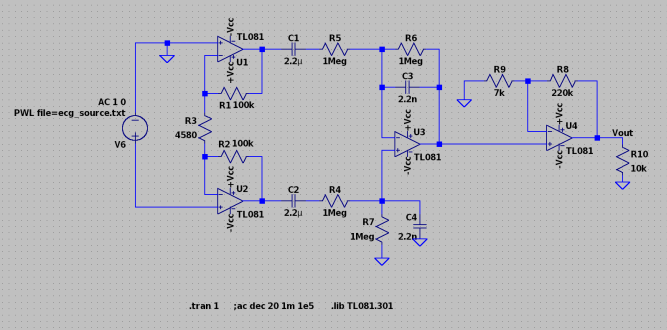
\includegraphics[width=\textwidth]{images/sim_crkt-fuente_ecg.png}
    \caption{Esquemático en LTspice con fuente \texttt{PWL file=ecg\_source.txt}.}
    \label{subfig:sim_crkt_ecg}
  \end{subfigure}
  \vspace{0.4cm}
  \begin{subfigure}[b]{0.88\textwidth}
    \centering
    \resizebox{\linewidth}{!}{%
      \begin{tikzpicture}
  \pgfplotsset{
    scale only axis,
    xmin=0, xmax=1.0,
  }
  \begin{axis}[
    width=0.80\textwidth,
    height=5.5cm,
    grid=both,
    grid style={line width=.1pt, draw=gray!25},
    major grid style={line width=.2pt, draw=gray!45},
    xlabel={Tiempo [\unit{\second}]},
    ylabel={Biopotencial de entrada $V_i$ [\unit{\milli\volt}]},
    ylabel style={color=red!80!black},
    yticklabel style={color=red!80!black},
    ymin=-2.0, ymax=8.4,
    ytick={-2, 0, 2, 4, 6, 8},
    axis y line*=left,
  ]
    \addplot[thick, dashed, color=red!80!black] table [x=time, y expr=\thisrow{vin}*1000] {sources/sim/sim_plot-fuente_ecg.txt};
  \end{axis}
  \begin{axis}[
    width=0.80\textwidth,
    height=5.5cm,
    ylabel={Tensión de salida $V_o$ [\unit{\volt}]},
    ylabel style={color=blue!80!black},
    yticklabel style={color=blue!80!black},
    ymin=-1.0, ymax=4.2,
    ytick={-1, 0, 1, 2, 3, 4},
    axis y line*=right,
    axis x line=none,
    legend style={at={(0.98,0.95)}, anchor=north east, font=\footnotesize}
  ]
    \addlegendimage{thick, dashed, color=red!80!black}
    \addlegendentry{Entrada $V_i$ [\unit{\milli\volt}]}
    \addplot[thick, color=blue!85!black] table [x=time, y=vout] {sources/sim/sim_plot-fuente_ecg.txt};
    \addlegendentry{Salida $V_o$ [\unit{\volt}]}
  \end{axis}
\end{tikzpicture}
%
    }
    \caption{Respuesta temporal al biopotencial cardíaco sintetizado.}
    \label{subfig:plot_sim_ecg}
  \end{subfigure}
  \caption{Simulación del circuito con señal electrocardiográfica.}
  \label{fig:sim_ecg_completa}
\end{figure}

Al inyectar una señal biopotencial diferencial de $V_{i,\text{pp}} \approx \SI{2.46}{\milli\volt\text{pp}}$ (con pico R de $\SI{2.04}{\milli\volt}$), la tensión de salida $V_o$ reproduce una forma de onda nítida de $V_{o,\text{pp}} \approx \SI{3.51}{\volt\text{pp}}$ (con pico R de $\SI{2.90}{\volt}$). Se comprueba:
\begin{enumerate}
  \item Preservación de la de la forma de onda QRS sin distorsión de flancos ni atenuación de altas frecuencias.
  \item Clara definición de las ondas lentas P y T.
  \item Eliminación absoluta de niveles de continua y centrado estable de la
      señal en $\SI{0}{\volt}$.
\end{enumerate}

% =========================================================================
% PARTE 2: ENSAYOS EXPERIMENTALES EN LABORATORIO
% =========================================================================
\clearpage
\section{Ensayos en laboratorio}
\label{subsec:ensayos_laboratorio}

Se procedió al diseño del amplificador en el programa KiCad (diseño de PCB
adjunto en anexo), a su montaje sobre una placa de circuito impreso
(Figura~\ref{fig:crkt_implementado}) y a su ensayo en laboratorio
(Figura~\ref{fig:medicion_lab}).

\begin{figure}[!ht]
  \centering
  \begin{subfigure}[b]{0.38\textwidth}
    \centering
    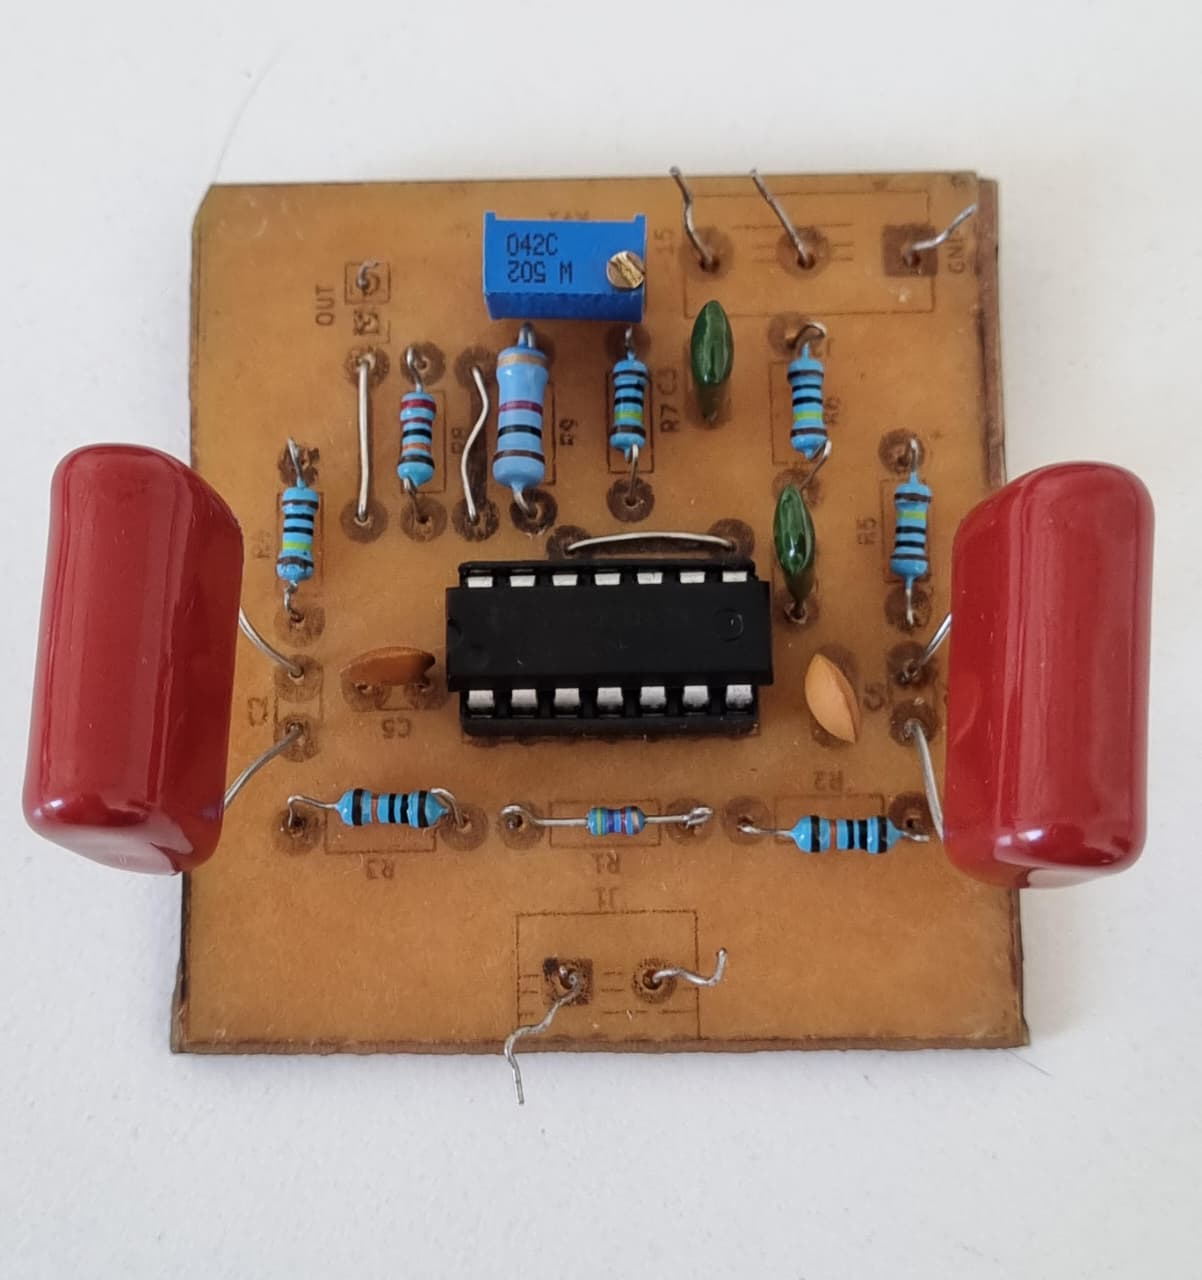
\includegraphics[height=4.6cm]{images/crkt_implementado.jpeg}
    \caption{Placa PCB ensamblada.}
    \label{fig:crkt_implementado}
  \end{subfigure}
  \hfill
  \begin{subfigure}[b]{0.58\textwidth}
    \centering
    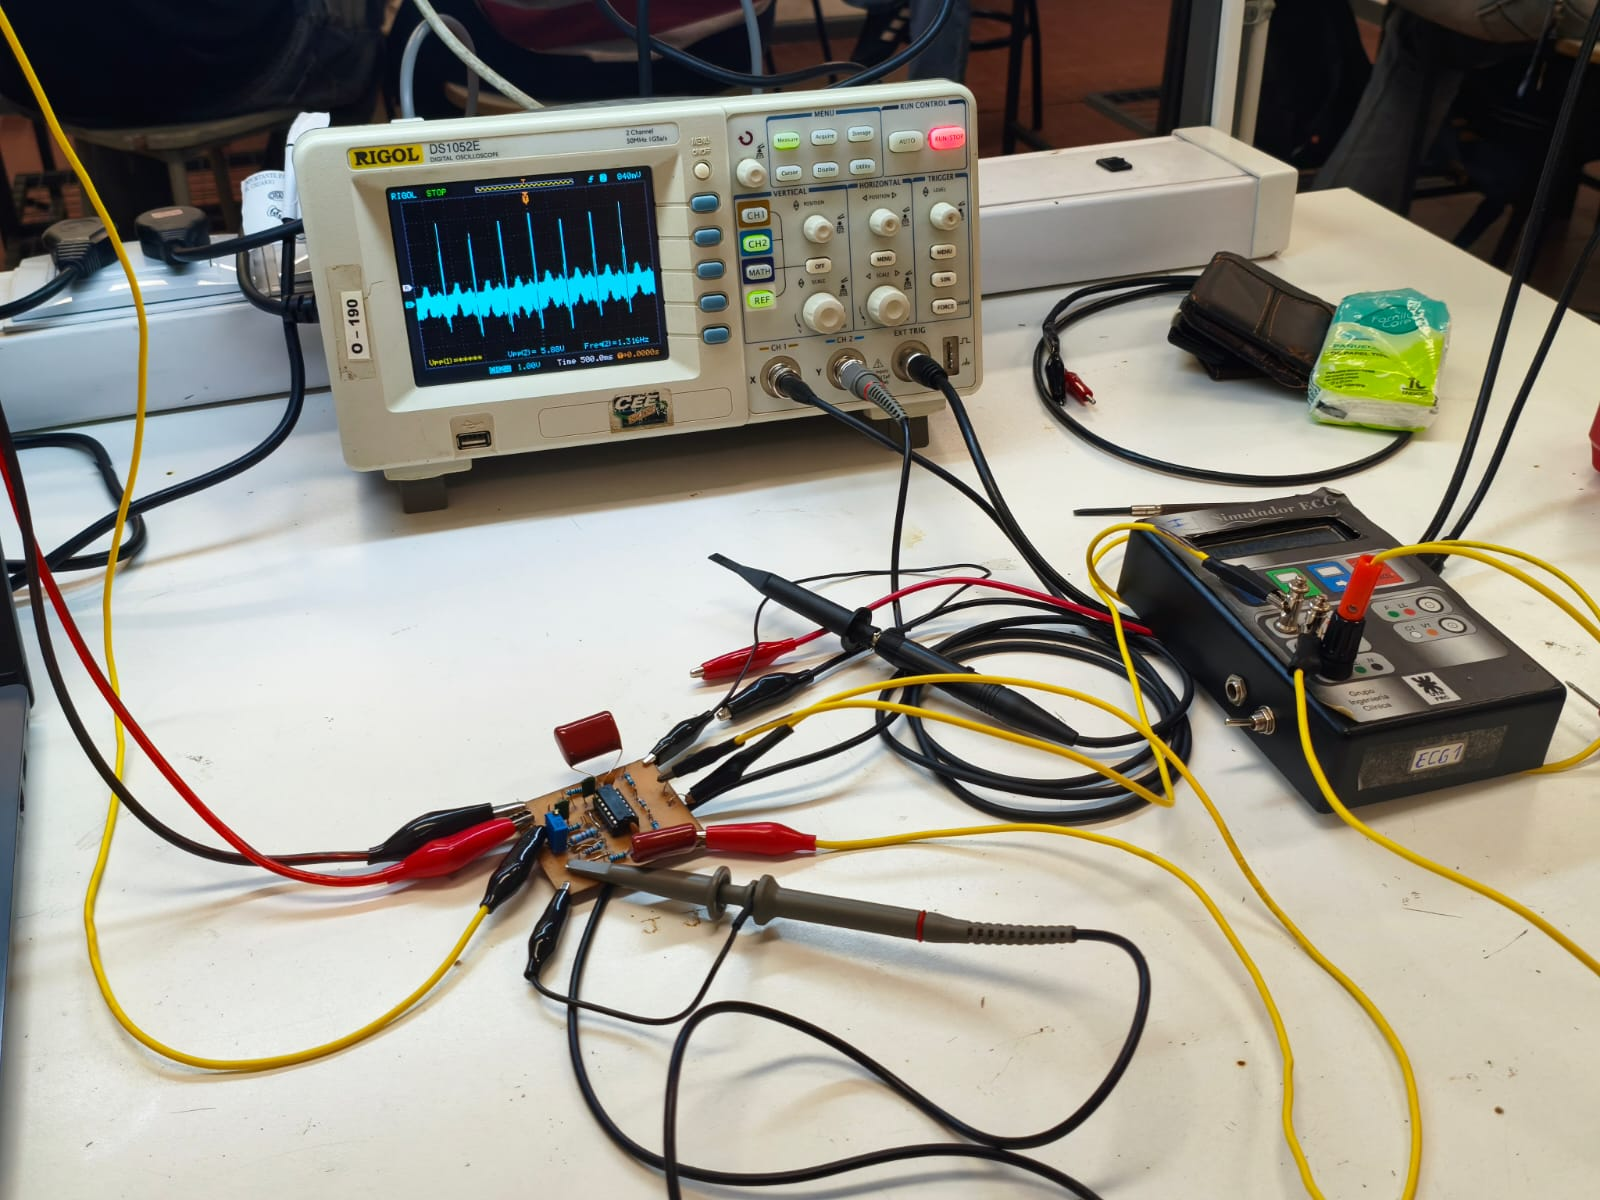
\includegraphics[height=4.6cm]{images/medicion_lab.jpeg}
    \caption{Ensayo experimental en banco de trabajo.}
    \label{fig:medicion_lab}
  \end{subfigure}
  \caption{Prototipo físico del amplificador de instrumentación: placa montada y puesta a prueba en banco de ensayo de laboratorio.}
  \label{fig:ensayo_prototipo}
\end{figure}

En las Figuras~\ref{crkt:medicion_rrmd}, \ref{crkt:medicion_rrmc} se detallan
las configuraciones instrumentales empleadas para los ensayos de modo
diferencial y modo común respectivamente.

\begin{figure}[!ht]
  \centering
  \begin{subfigure}[b]{0.48\textwidth}
    \centering
    \resizebox{\linewidth}{!}{%
      \begin{tikzpicture}[scale=0.95, transform shape]
  % Tarjeta exterior redondeada
  \draw[rounded corners=7pt, draw=gray!40, line width=0.8pt, fill=white] (-0.5, -0.3) rectangle (4.5, 2.7);

  % Triángulo Amplificador de Instrumentación (A.I.)
  \draw[line width=0.9pt] (1.9, 0.9) -- (1.9, 2.3) -- (2.8, 1.6) -- cycle;
  \node[font=\footnotesize\bfseries] at (2.2, 1.6) {A.I.};

  % Terminal superior (inversor) conectado a masa
  \draw[line width=0.7pt] (1.9, 2.1) -- (1.35, 2.1);
  \filldraw[black] (1.35, 2.1) circle (1.1pt);
  \draw[line width=0.7pt] (1.35, 2.1) -- (1.35, 1.6);

  % Terminal medio (referencia / masa)
  \draw[line width=0.7pt] (1.9, 1.6) -- (1.2, 1.6);
  % Masa de referencia del terminal medio
  \draw[line width=0.6pt] (1.2, 1.6) -- (1.2, 1.50);
  \draw[line width=0.8pt] (1.2-0.16, 1.50) -- (1.2+0.16, 1.50);
  \draw[line width=0.8pt] (1.2-0.10, 1.44) -- (1.2+0.10, 1.44);
  \draw[line width=0.8pt] (1.2-0.04, 1.38) -- (1.2+0.04, 1.38);

  % Terminal inferior (no inversor) conectado a generador
  \draw[line width=0.7pt] (1.9, 1.1) -- (0.65, 1.1) -- (0.65, 0.75);
  % Generador senoidal 10 mV, 25 Hz
  \draw[line width=0.7pt, fill=white] (0.65, 0.55) circle (0.18);
  \draw[line width=0.6pt] (0.65-0.11, 0.55) sin (0.65-0.055, 0.62) cos (0.65, 0.55) sin (0.65+0.055, 0.48) cos (0.65+0.11, 0.55);
  \node[anchor=west, align=left, font=\tiny] at (0.87, 0.55) {10 mV\\[-2pt]25Hz};
  % Masa del generador
  \draw[line width=0.7pt] (0.65, 0.37) -- (0.65, 0.30);
  \draw[line width=0.6pt] (0.65, 0.30) -- (0.65, 0.20);
  \draw[line width=0.8pt] (0.65-0.16, 0.20) -- (0.65+0.16, 0.20);
  \draw[line width=0.8pt] (0.65-0.10, 0.14) -- (0.65+0.10, 0.14);
  \draw[line width=0.8pt] (0.65-0.04, 0.08) -- (0.65+0.04, 0.08);

  % Salida Vo y Multímetro
  \draw[line width=0.7pt] (2.8, 1.6) -- (3.4, 1.6);
  \filldraw[black] (3.2, 1.6) circle (1.1pt);
  \node[above, font=\footnotesize] at (3.2, 1.63) {Vo};
  \draw[line width=0.7pt] (3.2, 1.6) -- (3.2, 1.18);

  % Símbolo de multímetro (voltímetro)
  \draw[line width=0.7pt, fill=white] (3.2, 0.95) circle (0.23);
  \node[font=\small\bfseries] at (3.2, 0.95) {V};
  \draw[-{Stealth[length=4pt, width=3pt]}, line width=0.5pt] (3.2-0.3, 0.95-0.3)
    -- (3.2+0.3, 0.95+0.3);

  % Masa del multímetro
  \draw[line width=0.7pt] (3.2, 0.72) -- (3.2, 0.60);
  \draw[line width=0.6pt] (3.2, 0.60) -- (3.2, 0.50);
  \draw[line width=0.8pt] (3.2-0.16, 0.50) -- (3.2+0.16, 0.50);
  \draw[line width=0.8pt] (3.2-0.10, 0.44) -- (3.2+0.10, 0.44);
  \draw[line width=0.8pt] (3.2-0.04, 0.38) -- (3.2+0.04, 0.38);
\end{tikzpicture}
%
    }
    \caption{Configuración para ganancia diferencial ($A_{md}$).}
    \label{crkt:medicion_rrmd}
  \end{subfigure}
  \hfill
  \begin{subfigure}[b]{0.48\textwidth}
    \centering
    \resizebox{\linewidth}{!}{%
      \begin{tikzpicture}[scale=0.95, transform shape]
  % Tarjeta exterior redondeada
  \draw[rounded corners=7pt, draw=gray!40, line width=0.8pt, fill=white] (-0.5, -0.3) rectangle (4.5, 2.7);

  % Triángulo Amplificador de Instrumentación (A.I.)
  \draw[line width=0.9pt] (1.9, 0.9) -- (1.9, 2.3) -- (2.8, 1.6) -- cycle;
  \node[font=\footnotesize\bfseries] at (2.2, 1.6) {A.I.};

  % Terminales de entrada unidos
  \draw[line width=0.7pt] (1.9, 2.1) -- (0.75, 2.1) -- (0.75, 1.1) -- (1.9, 1.1);
  \filldraw[black] (0.75, 1.4) circle (1.1pt);
  \draw[line width=0.7pt] (0.75, 1.4) -- (0.75, 0.75);

  % Terminal medio (referencia / masa)
  \draw[line width=0.7pt] (1.9, 1.6) -- (1.35, 1.6);
  % Masa de referencia del terminal medio
  \draw[line width=0.6pt] (1.35, 1.6) -- (1.35, 1.50);
  \draw[line width=0.8pt] (1.35-0.16, 1.50) -- (1.35+0.16, 1.50);
  \draw[line width=0.8pt] (1.35-0.10, 1.44) -- (1.35+0.10, 1.44);
  \draw[line width=0.8pt] (1.35-0.04, 1.38) -- (1.35+0.04, 1.38);

  % Generador senoidal en modo común
  \draw[line width=0.7pt, fill=white] (0.75, 0.55) circle (0.18);
  \draw[line width=0.6pt] (0.75-0.11, 0.55) sin (0.75-0.055, 0.62) cos (0.75, 0.55) sin (0.75+0.055, 0.48) cos (0.75+0.11, 0.55);
  \node[anchor=west, align=left, font=\tiny] at (0.97, 0.55) {1 Vpp\\[-2pt]25Hz};
  % Masa del generador
  \draw[line width=0.7pt] (0.75, 0.37) -- (0.75, 0.30);
  \draw[line width=0.6pt] (0.75, 0.30) -- (0.75, 0.20);
  \draw[line width=0.8pt] (0.75-0.16, 0.20) -- (0.75+0.16, 0.20);
  \draw[line width=0.8pt] (0.75-0.10, 0.14) -- (0.75+0.10, 0.14);
  \draw[line width=0.8pt] (0.75-0.04, 0.08) -- (0.75+0.04, 0.08);

  % Salida Vo y Multímetro
  \draw[line width=0.7pt] (2.8, 1.6) -- (3.4, 1.6);
  \filldraw[black] (3.2, 1.6) circle (1.1pt);
  \node[above, font=\footnotesize] at (3.2, 1.63) {Vo};
  \draw[line width=0.7pt] (3.2, 1.6) -- (3.2, 1.18);

  % Símbolo de multímetro (voltímetro)
  \draw[line width=0.7pt, fill=white] (3.2, 0.95) circle (0.23);
  \node[font=\small\bfseries] at (3.2, 0.95) {V};
  \draw[-{Stealth[length=4pt, width=3pt]}, line width=0.5pt] (3.2-0.3, 0.95-0.3)
    -- (3.2+0.3, 0.95+0.3);

  % Masa del multímetro
  \draw[line width=0.7pt] (3.2, 0.72) -- (3.2, 0.60);
  \draw[line width=0.6pt] (3.2, 0.60) -- (3.2, 0.50);
  \draw[line width=0.8pt] (3.2-0.16, 0.50) -- (3.2+0.16, 0.50);
  \draw[line width=0.8pt] (3.2-0.10, 0.44) -- (3.2+0.10, 0.44);
  \draw[line width=0.8pt] (3.2-0.04, 0.38) -- (3.2+0.04, 0.38);
\end{tikzpicture}
%
    }
    \caption{Configuración para ganancia en modo común ($A_{mc}$).}
    \label{crkt:medicion_rrmc}
  \end{subfigure}
  \caption{Esquemas instrumentales de conexión para la caracterización de rechazo de modo común en laboratorio.}
  \label{fig:setups_rrmc}
\end{figure}

\FloatBarrier
\subsection{Medición Experimental del RRMC}
La medición del Rechazo de Modo Común se efectuó inyectando señales a $\SI{25}{\hertz}$ (frecuencia central de la banda pasante, representativa de las perturbaciones de red de $\SI{50}{\hertz}$):
\begin{enumerate}
  \item \textbf{Modo Diferencial ($A_{md}$):} Con una entrada senoidal diferencial inyectada de $\SI{10}{\milli\volt}$, se midió una salida en el osciloscopio de $\SI{21.8}{\volt}$, resultando:
  \begin{equation*}
    A_{md,\text{med}} = \frac{\SI{21.8}{\volt}}{\SI{10}{\milli\volt}} = 2180.0\ \text{V/V} \equiv \SI{66.77}{\decibel}
  \end{equation*}
  \item \textbf{Modo Común ($A_{mc}$):} Con ambas entradas cortocircuitadas y excitadas con $\SI{1}{\volt}$, la tensión registrada a la salida fue de tan solo $\SI{25}{\milli\volt}$, arrojando:
  \begin{equation*}
    A_{mc,\text{med}} = \frac{\SI{25}{\milli\volt}}{\SI{1}{\volt}} = 0.0250\ \text{V/V} \equiv -\SI{32.04}{\decibel}
  \end{equation*}
  \item \textbf{RRMC experimental resultante:}
  \begin{equation*}
    \text{RRMC}_{\text{med}} = 20 \log_{10} \left( \frac{A_{md,\text{med}}}{A_{mc,\text{med}}} \right) = 20 \log_{10} \left( \frac{2180.0}{0.0250} \right) = 20 \log_{10}(87200) \approx \mathbf{\SI{98.80}{\decibel}}
  \end{equation*}
\end{enumerate}

En el Cuadro~\ref{tab:mediciones_rrmc} se encuentran los resultados
experimentales medidos frente a los valores obtenidos por simulación.

\begin{table}[!ht]
  \centering
  \caption{Comparativa de parámetros de modo diferencial, común y RRMC: valores simulados vs.\ mediciones experimentales en laboratorio.}
  \label{tab:mediciones_rrmc}
  \resizebox{\textwidth}{!}{%
  \begin{tabular}{|l|c|c|c|c|c|c|}
    \hline
    Parámetro de Ensayo & Frecuencia & $V_{\text{in}}$ aplicado & $V_{\text{out}}$ simulado & Ganancia Sim. & $V_{\text{out}}$ medido & Ganancia Medida \\ \hline
    Modo Diferencial ($A_{md}$) & $\SI{25}{\hertz}$ & $\SI{10}{\milli\volt}$ & $\SI{13.36}{\volt}$ & $1336.3\ \text{V/V}$ ($\SI{62.52}{\decibel}$) & $\SI{21.8}{\volt}$ & $2180.0\ \text{V/V}$ ($\SI{66.77}{\decibel}$) \\ \hline
    Modo Común ($A_{mc}$) & $\SI{25}{\hertz}$ & $\SI{1}{\volt}$ & $\SI{0.84}{\milli\volt}$ & $8.36 \times 10^{-4}$ ($-\SI{61.55}{\decibel}$) & $\SI{25}{\milli\volt}$ & $0.0250\ \text{V/V}$ ($-\SI{32.04}{\decibel}$) \\ \hline
    \multicolumn{3}{|l|}{\textbf{RRMC resultante (\unit{\decibel})}} & \multicolumn{2}{c|}{$\mathbf{\SI{124.07}{\decibel}}$ (Simulado)} & \multicolumn{2}{c|}{$\mathbf{\SI{98.80}{\decibel}}$ (Medido en laboratorio)} \\ \hline
  \end{tabular}%
  }
\end{table}

El valor medido de $\mathbf{\SI{98.80}{\decibel}}$ supera con amplio margen la
especificación mínima requerida ($\text{RRMC} \gg \SI{80}{\decibel}$). La
divergencia observada respecto al valor de simulación ($\SI{124.07}{\decibel}$)
se debe a que, mientras la simulación asume componentes ideales, en la placa
real las tolerancias y factores parásitos limita el RRMC práctico.

\subsection{Relevamiento Experimental de Respuesta en Frecuencia y Ancho de Banda}
Se ejecutó un barrido sinusoidal diferencial manteniendo la tensión de entrada constante en $V_{\text{in}} = \SI{10}{\milli\volt}$ en 21 frecuencias discretas distribuidas entre $\SI{0.1}{\hertz}$ y $\SI{2}{\kilo\hertz}$.

En el Cuadro~\ref{tab:barrido_frecuencia} se presenta el registro experimental completo obtenido en el laboratorio para el barrido en frecuencia, expresando la variación $\Delta$ en decibeles respecto a la frecuencia central de $\SI{25}{\hertz}$. El contraste con la respuesta teórica de simulación circuital se evalúa y visualiza en el diagrama de Bode comparativo de la Figura~\ref{fig:sim_bode_pgf}.

\begin{table}[!ht]
  \centering
  \renewcommand{\arraystretch}{1.12}
  \caption{Relevamiento experimental del barrido en frecuencia medido en laboratorio ($V_{\text{in}} = \SI{10}{\milli\volt}$).}
  \label{tab:barrido_frecuencia}
  \begin{tabular}{|c|c|c|c|c|}
    \hline
    $f$ (\unit{\hertz}) & $V_{\text{in}}$ (\unit{\milli\volt}) & $V_o$ medido (\unit{\volt}) & Ganancia (\unit{\decibel}) & $\Delta$ vs.\ $\SI{25}{\hertz}$ med. (\unit{\decibel}) \\ \hline
    0.1  & 10 & 19.00 & 65.58 & -1.19 \\ \hline
    0.25 & 10 & 22.80 & 67.16 & +0.39 \\ \hline
    0.5  & 10 & 23.60 & 67.46 & +0.69 \\ \hline
    1    & 10 & 23.60 & 67.46 & +0.69 \\ \hline
    2    & 10 & 23.60 & 67.46 & +0.69 \\ \hline
    5    & 10 & 23.60 & 67.46 & +0.69 \\ \hline
    10   & 10 & 23.40 & 67.38 & +0.62 \\ \hline
    20   & 10 & 22.80 & 67.16 & +0.39 \\ \hline
    25   & 10 & 21.80 & 66.77 & +0.00 \\ \hline
    50   & 10 & 19.60 & 65.85 & -0.92 \\ \hline
    75   & 10 & 16.40 & 64.30 & -2.47 \\ \hline
    100  & 10 & 13.50 & 62.61 & -4.16 \\ \hline
    125  & 10 & 11.60 & 61.29 & -5.48 \\ \hline
    150  & 10 & 10.00 & 60.00 & -6.77 \\ \hline
    200  & 10 & 8.00  & 58.06 & -8.71 \\ \hline
    300  & 10 & 5.30  & 54.49 & -12.28 \\ \hline
    500  & 10 & 3.32  & 50.42 & -16.35 \\ \hline
    700  & 10 & 2.32  & 47.31 & -19.46 \\ \hline
    1000 & 10 & 1.56  & 43.86 & -22.91 \\ \hline
    1500 & 10 & 1.10  & 40.83 & -25.94 \\ \hline
    2000 & 10 & 0.82  & 38.28 & -28.49 \\ \hline
  \end{tabular}
\end{table}

\clearpage

En la Figura~\ref{fig:sim_bode_pgf} se superponen los 21 puntos experimentales
medidos  sobre la curva de simulación, permitiendo verificar visualmente el
los resultados obtenidos.

\begin{figure}[!ht]
  \centering
  \begin{tikzpicture}
  \begin{axis}[
    width=0.96\textwidth,
    height=8.5cm,
    xmode=log,
    xmin=1e-2, xmax=3e3,
    ymin=20, ymax=85,
    ytick={20, 30, 40, 50, 60, 70, 80},
    grid=both,
    grid style={line width=.1pt, draw=gray!25},
    major grid style={line width=.2pt, draw=gray!45},
    xlabel={Frecuencia [\unit{\hertz}]},
    ylabel={Ganancia $|A_v|$ [\unit{\decibel}]},
    legend style={at={(0.98,0.96)}, anchor=north east, font=\footnotesize}
  ]
    % Curva simulada
    \addplot[very thick, color=blue!85!black] table [x=freq, y=gain_db] {sources/sim/sim_plot-rta_frec.txt};
    \addlegendentry{Respuesta simulada $|A_v(f)|$}

    % Puntos medidos en laboratorio
    \addplot[only marks, mark=*, mark size=2pt, color=red!80!black] coordinates {
      (0.1, 65.58)
      (0.25, 67.16)
      (0.5, 67.46)
      (1, 67.46)
      (2, 67.46)
      (5, 67.46)
      (10, 67.38)
      (20, 67.16)
      (25, 66.77)
      (50, 65.85)
      (75, 64.30)
      (100, 62.61)
      (125, 61.29)
      (150, 60.00)
      (200, 58.06)
      (300, 54.49)
      (500, 50.42)
      (700, 47.31)
      (1000, 43.86)
      (1500, 40.83)
      (2000, 38.28)
    };
    \addlegendentry{Medición en laboratorio}

    % Linea de referencia -3 dB simulada (60.2 dB)
    \addplot[dashed, thick, color=blue!70!gray, domain=1e-2:3e3] {60.21};
    \addlegendentry{Nivel sim. $-\SI{3}{\decibel}$ ($\SI{60.2}{\decibel}$)}

    % Lineas verticales en fL y fH simuladas
    \draw[dotted, thick, color=blue!80!black] (axis cs:0.0725, 20) -- (axis cs:0.0725, 60.21);
    \node[anchor=south west, font=\scriptsize, rotate=90, color=blue!80!black] at (axis cs:0.0725, 22) {$f_{L,\text{sim}} \approx \SI{0.07}{\hertz}$};

    % Linea vertical fH simulada (72.3 Hz)
    \draw[dotted, thick, color=blue!80!black] (axis cs:72.32, 20) -- (axis cs:72.32, 60.21);
    \node[anchor=south west, font=\scriptsize, rotate=90, color=blue!80!black] at (axis cs:72.32, 23) {$f_{H,\text{sim}} \approx \SI{72.3}{\hertz}$};

    % Linea vertical fH medida (82.2 Hz)
    \draw[dotted, thick, color=red!80!black] (axis cs:82.2, 20) -- (axis cs:82.2, 63.77);
    \node[anchor=north west, font=\scriptsize, rotate=90, color=red!80!black] at (axis cs:82.2, 23) {$f_{H,\text{med}} = \SI{82.2}{\hertz}$};
  \end{axis}
\end{tikzpicture}
%
  \caption{Bode $|A_v(f)|$: curva de simulación vs puntos medidos en laboratorio.}
  \label{fig:sim_bode_pgf}
\end{figure}

A partir del relevamiento experimental se comprueban los siguientes parámetros frente a los valores esperados:
\begin{itemize}
  \item \textbf{Ganancia en banda de paso:} La ganancia central a $\SI{25}{\hertz}$ fue de $\SI{66.77}{\decibel}$ ($2180.0\ \text{V/V}$), alcanzando una cota máxima plana de $\SI{67.46}{\decibel}$ ($2360.0\ \text{V/V}$) entre $\SI{0.5}{\hertz}$ y $\SI{5}{\hertz}$. Ambas superan holgadamente la cota mínima de diseño impuesta de $\ge \SI{60}{\decibel}$ ($1000\ \text{V/V}$).
  \item \textbf{Frecuencia de corte inferior ($f_L$):} Se corroboró que a $\SI{0.1}{\hertz}$ la respuesta ya se encuentra plenamente dentro de la banda útil ($\SI{65.58}{\decibel}$, con solo $-\SI{1.19}{\decibel}$ de atenuación respecto a $\SI{25}{\hertz}$), validando el bloqueo de continua y concordando con el polo teórico esperado de $f_L \approx \SI{0.07}{\hertz}$.
  \item \textbf{Frecuencia de corte superior ($f_H$):} La atenuación a $-\SI{3}{\decibel}$ respecto a la ganancia central ($\SI{66.77}{\decibel} - \SI{3.00}{\decibel} = \SI{63.77}{\decibel}$) se determinó experimentalmente en:
  \begin{equation*}
    f_{H,\text{med}} = \mathbf{\SI{82.2}{\hertz}}
  \end{equation*}
  La discrepancia del $+13.7\%$ frente al valor nominal esperado ($\SI{72.3}{\hertz}$) resulta totalmente justificada por la tolerancia comercial de los capacitores de poliéster ($C_4 = \SI{2.2}{\nano\farad} \pm 10\%$) y la dispersión resistiva.
  \item \textbf{Ancho de banda efectivo:} El ancho de banda medido resulta $\text{BW}_{\text{med}} = \mathbf{\SI{82.2}{\hertz}}$, cumpliendo con creces la banda requerida para el registro electrocardiográfico ($\SI{0.05}{\hertz}$ a $\SI{100}{\hertz}$).
\end{itemize}

\clearpage
\subsection{Síntesis y Comprobación frente a las Especificaciones de Diseño}
En el Cuadro~\ref{tab:sintesis_especificaciones} se resume la contrastación final entre los requerimientos de partida, los resultados calculados analíticamente, las simulaciones circuitales y las mediciones experimentales en laboratorio.

\begin{table}[!ht]
  \centering
  \caption{Síntesis comparativa final: especificaciones impuestas vs.\ cálculos analíticos, simulación en LTspice y mediciones de laboratorio.}
  \label{tab:sintesis_especificaciones}
  \resizebox{0.95\textwidth}{!}{%
  \begin{tabular}{|l|c|c|c|c|c|}
    \hline
    Parámetro de Diseño & Especificación & Cálculo Teórico & Simulación LTspice & Medición Laboratorio & Estado \\ \hline
    Ganancia diferencial ($A_{md}$) & $\ge \SI{60}{\decibel}$ ($1000\times$) & $\SI{63.00}{\decibel}$ ($1413\times$) & $\SI{62.52}{\decibel}$ ($1336\times$) & $\SI{66.77}{\decibel}$ ($2180\times$) & \textbf{Cumple} \\ \hline
    Frecuencia de corte inferior ($f_L$) & $0.05\text{ a } \SI{0.07}{\hertz}$ & $\SI{0.072}{\hertz}$ & $\SI{0.072}{\hertz}$ & Activo en $\SI{0.1}{\hertz}$ & \textbf{Cumple} \\ \hline
    Frecuencia de corte superior ($f_H$) & $70\text{ a } \SI{100}{\hertz}$ & $\SI{72.34}{\hertz}$ & $\SI{72.32}{\hertz}$ & $\SI{82.20}{\hertz}$ & \textbf{Cumple} \\ \hline
    Ancho de banda pasante ($\text{BW}$) & $70\text{ a } \SI{100}{\hertz}$ & $\SI{72.27}{\hertz}$ & $\SI{72.25}{\hertz}$ & $\SI{82.20}{\hertz}$ & \textbf{Cumple} \\ \hline
    Rechazo de Modo Común (RRMC) & $\gg \SI{80}{\decibel}$ & $\infty$ (ideal) & $\SI{124.07}{\decibel}$ & $\mathbf{\SI{98.80}{\decibel}}$ & \textbf{Cumple} \\ \hline
    Rechazo de continua ($A_v(0)$) & $\SI{0}{\decibel}$ (bloqueo) & $0\ \text{V/V}$ ($-\infty\ \text{dB}$) & $0\ \text{V/V}$ ($-\infty\ \text{dB}$) & Verificado ($V_{\text{offset}} \approx 0$) & \textbf{Cumple} \\ \hline
  \end{tabular}%
  }
\end{table}

Como balance general del proceso de validación, se comprueba que el prototipo
físico no solo satisface la totalidad de las pautas de diseño estipuladas, sino
que exhibe un desempeño altamente robusto frente a perturbaciones externas. La
concordancia cualitativa y cuantitativa entre el análisis analítico, el
comportamiento simulado en LTspice y las curvas relevadas en el banco
experimental demuestra la validez del diseño.

\chapter{Conclusiones}
\label{sec:conclusiones}

El presente trabajo abordó el diseño analítico, la simulación circuital y la
validación experimental en laboratorio de un sistema de acondicionamiento para
señales electrocardiográficas (ECG). La arquitectura desarrollada integró un
amplificador de instrumentación de tres amplificadores operacionales con
filtrado pasabanda activo en su propia etapa restadora, complementado con una
etapa final de post-amplificación y calibración. En lo relativo a la ganancia
diferencial, la implementación cumplió holgadamente la cota impuesta ($\ge
\SI{60}{\decibel}$): 
se registró una ganancia de $\SI{66.77}{\decibel}$ ($2180.0\ \text{V/V}$) a
$\SI{25}{\hertz}$. Esta amplificación transforma señales cardíacas débiles
($\sim \SI{1}{\milli\volt\text{pp}}$ a $\SI{2.5}{\milli\volt\text{pp}}$) en
amplitudes de $\SI{2}{\volt}$ a $\SI{3.5}{\volt\text{pp}}$, ideales
para su digitalización sin distorsión armónica apreciable.

La incorporación de reactancias en la etapa restadora resultó altamente eficaz
para la selectividad espectral del circuito, suprimiendo la necesidad de etapas
de filtrado adicionales. La función de transferencia presentó un cero en el
origen que garantizó ganancia nula a corriente continua ($A_v(0) = 0$),
confiriendo inmunidad absoluta frente a potenciales galvánicos de contacto
electrodo-piel (hasta $\pm \SI{300}{\milli\volt}$) y suprimiendo cualquier
corrimiento de línea de base. Asimismo, el polo inferior en $f_L \approx
\SI{0.07}{\hertz}$ y el corte superior nominal en $f_{H,\text{sim}} \approx
\SI{72.3}{\hertz}$ se contrastaron con la placa física, donde se midió un corte
experimental de $f_{H,\text{med}} = \mathbf{\SI{82.2}{\hertz}}$ y un ancho de
banda efectivo de $\mathbf{\SI{82.2}{\hertz}}$, plenamente apto para el
monitoreo ECG. 

En cuanto a la inmunidad frente a ruidos de modo común, el prototipo físico
alcanzó un $\text{RRMC}_{\text{med}} = \mathbf{\SI{98.80}{\decibel}}$ a
$\SI{25}{\hertz}$ ($A_{md} = 2180.0\ \text{V/V}$ y $A_{mc} = 0.0250\
\text{V/V}$), superando con holgura la especificación exigida ($\gg
\SI{80}{\decibel}$). Este resultado asegura una eliminación contundente de las
interferencias de red de $\SI{50}{\hertz}$. Por último, la elección de
amplificadores BiFET (TL084) fue plenamente acertada: su elevada impedancia de
entrada  y sus corrientes de polarización mínimas, sumando su disponibilidad en
tiendas locales de electrónica y su buen costo económico contribuyeron a la
satifactoria realización del trabajo práctico. En conjunto, la estrecha
correlación entre cálculo teórico, simulación y mediciones sobre PCB valida la
robustez, compacidad y viabilidad del diseño propuesto.


% Bibliografía
\nocite{*}
\printbibliography[heading=bibnumbered, title={Fuentes}]

% Anexos
\chapter{Anexos}
\label{sec:anexos}

\section{Directivas y Parámetros de Simulación en LTspice}

Para la validación circuital en el software LTspice se emplearon los modelos SPICE provistos por los fabricantes para
el operacional TL081 (librería \texttt{TL081.301}) y modelos comparativos (\texttt{op07.lib}).

\begin{lstlisting}[style=ltspice, caption={Directivas SPICE empleadas para la caracterización en frecuencia y en el dominio temporal.}]
* Analisis de respuesta en frecuencia (Diagrama de Bode)
.ac dec 20 1m 100k

* Analisis transitorio con senal cardiaca sintetizada
.tran 0 2 0 100u

* Definicion de la fuente biopotencial ECG desde archivo de texto
V_ecg in_p in_m PWL file=ecg_source.txt

* Inclusion de modelos de amplificadores operacionales
.lib TL081.301
.lib op07.lib
\end{lstlisting}

\section{Protocolo de Calibración en Laboratorio}

Para la puesta a punto experimental del instrumento se recomienda el siguiente procedimiento secuencial:
\begin{enumerate}
  \item Verificación de polarización estática:
  Conectar las fuentes de alimentación partidas a $\pm \SI{12}{\volt}$ o $\pm \SI{15}{\volt}$. Cortocircuitar ambas
  entradas a masa ($e_1 = e_2 = \SI{0}{\volt}$) y comprobar con el multímetro que la tensión en la salida $V_o$ sea
  inferior a $\SI{10}{\milli\volt}$ en continua.
  \item Calibración de la ganancia de primera y segunda etapa:
  Inyectar en la entrada diferencial una señal senoidal de $\SI{10}{\milli\volt}$ de amplitud ($\SI{20}{\milli\volt\text{pp}}$) a $\SI{25}{\hertz}$. Con el
  osciloscopio monitoreando la salida de $U_3$, ajustar el trimpot $R_1$ hasta observar una ganancia intermedia de $44.67\ \text{V/V}$ ($\approx \SI{33.0}{\decibel}$, correspondiente a $\approx \SI{0.89}{\volt\text{pp}}$).
  \item Calibración de la ganancia global de salida:
  Trasladar la sonda del osciloscopio al terminal de salida final $V_o$. Sin alterar la señal de entrada, ajustar el
  trimpot de salida $R_9$ hasta obtener la ganancia total del sistema de diseño ($\approx 1336\ \text{V/V} \equiv \SI{62.5}{\decibel}$ a $\SI{25}{\hertz}$, con $V_o \approx \SI{26.7}{\volt\text{pp}}$ sin saturación dentro de la zona lineal de alimentación).
  \item Verificación con simulador cardíaco:
  Conectar el generador de bioseñales virtuales configurado en modo QRS adulto ($1\ \text{mVpp}$ a $60\ \text{bpm}$).
  Comprobar que en la pantalla del osciloscopio la señal exhiba una amplitud de $\SI{1}{\volt\text{pp}}$ con línea de base
  estable en cero voltios.
\end{enumerate}


\end{document}
